% ============================================================
% 生物医学图像处理 — 期末大作业 实验报告
% Project 2: 皮肤镜图像病变分类
% ============================================================
\documentclass[UTF8,a4paper,12pt]{ctexart}

% ---- 页面布局 ----
\usepackage[top=2.5cm, bottom=2.5cm, left=2.8cm, right=2.8cm]{geometry}

% ---- 数学公式 ----
\usepackage{amsmath,amssymb}

% ---- 图表支持 ----
\usepackage{graphicx}
\usepackage{float}
\usepackage{subcaption}
\usepackage{booktabs}
\usepackage{longtable}
\usepackage{array}
\usepackage{multirow}

% ---- 超链接与引用 ----
\usepackage[colorlinks=true,
            linkcolor=blue,
            citecolor=blue,
            urlcolor=blue]{hyperref}

% ---- 算法伪代码 ----
\usepackage{algorithm}
\usepackage{algpseudocode}
\floatname{algorithm}{算法}

% ---- 代码排版 ----
\usepackage{listings}
\usepackage{xcolor}
\lstset{
    basicstyle=\ttfamily\small,
    breaklines=true,
    frame=single,
    numbers=left,
    numberstyle=\tiny,
    backgroundcolor=\color{gray!5},
    tabsize=2,
}

% ---- 图表编号关联章节 ----
\numberwithin{figure}{section}
\numberwithin{table}{section}

% ---- 自定义命令 ----
\newcommand{\tabincell}[2]{\begin{tabular}{@{}#1@{}}#2\end{tabular}}
\newcommand{\imgwidth}{0.48\textwidth}

% ====================== 文档信息 ======================
\title{\textbf{生物医学图像处理期末大作业实验报告 \\[6pt]
        \large Project 2: 基于传统机器学习与深度学习的 \\ 皮肤镜图像病变分类}}
\author{Project 2 小组}
\date{\today}

\begin{document}

\maketitle
\thispagestyle{empty}

% ====================== 摘要 ======================
\begin{abstract}
\noindent 本报告围绕\textbf{Project 2：皮肤镜图像病变分类}任务，系统阐述了从数据预处理、手工特征提取到传统机器学习模型训练与评估，再到深度学习迁移学习对比以及鲁棒性分析的完整技术流程。针对黑色素瘤（melanoma, mel）、普通痣（nevus, nv）和血管病变（vascular lesion, vasc）三类皮肤镜图像，项目构建了两套互补方案：基于127维手工特征（颜色矩、颜色直方图、GLCM纹理、LBP纹理）的传统机器学习分类器（SVM、随机森林、KNN），以及基于卷积神经网络（ResNet-18、MobileNetV2）的深度学习补充方案。

\noindent 实验结果表明：传统方法中，随机森林取得最佳测试准确率\textbf{73.33\%}（Macro-F1=0.736），SVM性能相当（72.50\%，Macro-F1=0.736），KNN较弱（66.67\%，Macro-F1=0.672）。深度学习方案中，MobileNetV2以\textbf{83.33\%}准确率和\textbf{0.840} Macro-F1显著超越传统方法（提升约10个百分点），在增强图子集上以79.1\%准确率优于传统随机森林（71.4\%）和ResNet18（75.8\%）。严格分组划分实验揭示了原增强划分中存在病灶级信息泄漏（198个训练编号与100个测试编号重叠98个），严格分组下随机森林Macro-F1降至0.578。报告还包含10种图像扰动下的鲁棒性测试、特征组消融实验和mel/nv混淆分析，全面论证了方法的有效性、局限性与改进方向。

\vspace{12pt}
\noindent\textbf{关键词：}皮肤镜图像分类；特征工程；机器学习；迁移学习；鲁棒性分析；医学图像处理
\end{abstract}

\newpage

% ====================== 目录 ======================
\tableofcontents
\newpage

% ====================== 第1章 引言 ======================
\section{引言}

\subsection{研究背景与意义}

皮肤癌是全球最常见的恶性肿瘤之一，其中黑色素瘤（melanoma）虽然发病率仅占皮肤癌的约1\%，却导致了绝大多数皮肤癌死亡病例。早期发现和准确诊断是提高患者生存率的关键。皮肤镜（dermoscopy）作为一种非侵入性的成像技术，通过消除皮肤表面反射并放大皮下结构，能够显著提高临床诊断的准确率。

然而，皮肤镜图像的解读高度依赖医生的经验，且不同病变类型（如黑色素瘤与良性痣）在视觉上高度相似，给人工诊断带来了巨大挑战。因此，开发计算机辅助诊断（Computer-Aided Diagnosis, CAD）系统，自动提取皮肤镜图像特征并进行准确分类，具有重要的临床意义。

\subsection{项目任务描述}

本项目（Project 2）的核心任务是：从皮肤镜图像中提取图像特征，使用机器学习方法对三类皮肤病变进行自动分类，并通过增强图像的识别表现来证明算法的鲁棒性。具体数据规模为200张原始皮肤镜图像，以及通过旋转、翻转生成的400张增强图像，共计600张图像。

根据课程要求，第15周定量评估采用传统图像处理方法与简单机器学习方法，严禁使用深度学习模型或外部数据。本章所述深度学习迁移学习方案，仅为课堂展示与课程报告的\textbf{补充对比}，不作为定量评估依据。

项目共由五名成员协作完成，涵盖以下五个模块：
\begin{enumerate}
    \item \textbf{数据预处理}：图像去噪、去毛发、尺寸归一化、亮度归一化、数据集划分；
    \item \textbf{特征工程}：颜色特征（颜色矩、颜色直方图）与纹理特征（GLCM、LBP）的提取、归一化、PCA降维及特征有效性分析；
    \item \textbf{模型训练与评估}：基于SVM、随机森林、KNN三种传统机器学习模型的训练、网格搜索参数调优及全面评估；
    \item \textbf{鲁棒性分析}：增强图像一致性检验、图像扰动鲁棒性测试、严格分组划分的稳定性分析；
    \item \textbf{深度学习对比实验}：使用ResNet-18/MobileNetV2迁移学习作为传统方法的补充对比和性能上界参考。
\end{enumerate}

\subsection{报告结构}

本报告剩余部分组织如下：第\ref{sec:data}节介绍数据集与预处理流程；第\ref{sec:feature}节详述特征提取方法；第\ref{sec:ml}节和第\ref{sec:dl}节分别介绍传统机器学习与深度学习方法；第\ref{sec:results}节展示了全面的实验结果；第\ref{sec:robustness}节进行鲁棒性分析；第\ref{sec:discussion}节展开深入讨论；第\ref{sec:conclusion}节总结全文。

% ====================== 第2章 数据与预处理 ======================
\section{数据集与预处理}\label{sec:data}

\subsection{数据概览}

原始数据集包含200张皮肤镜图像，按照80/20比例分层划分为训练集和测试集。为增强模型泛化能力和评估鲁棒性，每张原始图像通过旋转（90°、180°、270°）和水平/垂直翻转生成2张增强变体（\_aug1、\_aug2），总计600张图像（480张训练+120张测试）。

三类病变的分布情况如表\ref{tab:data_dist}所示。数据存在中等程度的类别不平衡：普通痣（nv）是多数类（约占50\%），血管病变（vasc）是少数类（约占15\%）。

\begin{table}[H]
\centering
\caption{数据集类别分布}
\label{tab:data_dist}
\begin{tabular}{lrrr}
\toprule
\textbf{类别} & \textbf{训练集} & \textbf{测试集} & \textbf{合计} \\
\midrule
黑色素瘤 (mel) & 168 & 42 & 210 \\
普通痣 (nv)    & 240 & 60 & 300 \\
血管病变 (vasc) & 72  & 18 & 90  \\
\midrule
\textbf{合计}  & \textbf{480} & \textbf{120} & \textbf{600} \\
\bottomrule
\end{tabular}
\end{table}

\subsection{预处理流程}

数据预处理包含以下关键步骤：

\paragraph{图像去噪} 采用非局部均值去噪（Non-Local Means Denoising）算法，在保持边缘和纹理细节的同时有效去除图像噪声。该算法利用图像的自相似性，对每个像素通过加权平均其邻域内的相似块进行去噪，相比高斯滤波能更好地保护皮肤镜图像中的精细结构。

\paragraph{毛发去除} 皮肤镜图像中可能存在的毛发会干扰特征提取，因此采用形态学黑帽变换（Black-Hat Transform）结合阈值化处理和图像修复（Inpainting）来检测并移除毛发区域。具体步骤为：首先通过黑帽变换突出暗色线状结构（毛发），然后通过阈值分割生成毛发掩膜，最后利用快速行进法（Fast Marching Method）对毛发区域进行修复填充。

\paragraph{尺寸归一化} 将所有图像缩放至统一尺寸256×256像素，确保后续特征提取的一致性和可比性。缩放采用双线性插值以保持图像平滑。

\paragraph{亮度归一化} 采用直方图均衡化（Histogram Equalization）或自适应直方图均衡化（CLAHE）对图像亮度进行归一化处理，减少不同采集条件下的光照差异对特征提取的影响。

\paragraph{数据集划分} 按图像原始ID（去除\_aug后缀）进行分组后分层划分，确保同一原始图像的原图和所有增强变体属于同一个划分（全在训练集或全在测试集），避免数据泄漏。

% ====================== 第3章 特征工程 ======================
\section{特征工程}\label{sec:feature}

图像特征的提取与表示是传统机器学习方法的核心。本节详述127维手工特征体系，涵盖颜色特征和纹理特征两大类别。

\subsection{颜色特征}

\subsubsection{颜色矩（Color Moments）}

颜色矩是一种紧凑且有效的颜色特征描述方法。对RGB三个通道分别计算一阶矩（均值）、二阶矩（标准差）和三阶矩（偏度），共计$3 \times 3 = 9$维特征。

对于通道$c$的$N$个像素值$\{p_i\}_{i=1}^{N}$，各阶矩定义为：

\begin{align}
\text{一阶矩（均值）:}\quad & \mu_c = \frac{1}{N}\sum_{i=1}^{N} p_i \\
\text{二阶矩（标准差）:}\quad & \sigma_c = \sqrt{\frac{1}{N}\sum_{i=1}^{N} (p_i - \mu_c)^2} \\
\text{三阶矩（偏度）:}\quad & s_c = \frac{1}{N}\sum_{i=1}^{N} \left(\frac{p_i - \mu_c}{\sigma_c}\right)^3
\end{align}

颜色矩的优势在于计算简单、维度低，且对于图像的旋转和平移具有一定的不变性。生理学上，不同皮肤病变类型的色素沉着程度和颜色分布存在差异，颜色矩可以有效捕捉这些宏观统计特性。

\subsubsection{颜色直方图（Color Histogram）}

颜色直方图描述了图像中各颜色强度的分布情况。对RGB三个通道分别计算32个等宽区间的归一化直方图，共计$3 \times 32 = 96$维特征：

\begin{equation}
h_c(b) = \frac{1}{N} \sum_{i=1}^{N} \mathbb{I}[p_i \in \text{bin}_b], \quad b = 1, 2, \ldots, 32
\end{equation}

其中$\mathbb{I}[\cdot]$为指示函数。归一化确保了不同尺寸图像的直方图具有可比性。直方图特征能够刻画图像颜色的整体分布模式，弥补了颜色矩仅描述低阶统计量而缺乏分布细节的不足。

\subsection{纹理特征}

纹理是皮肤镜图像中判别病变类型的关键信息，不同病变呈现不同的纹理模式（如网状、点状、球状等）。

\subsubsection{灰度共生矩阵（GLCM）}

灰度共生矩阵（Gray-Level Co-occurrence Matrix）通过统计图像中特定距离和方向上像素对的出现频率来描述纹理的空间依赖关系。设图像灰度级为$L=256$，在距离$d$和方向$\theta$下的GLCM定义为：

\begin{equation}
P(i, j \mid d, \theta) = \#\{(x,y) \mid I(x,y)=i,\; I(x+dx, y+dy)=j\}
\end{equation}

其中$dx = d \cdot \cos\theta$，$dy = d \cdot \sin\theta$。

本项目使用2个距离（$d=1,2$）和4个方向（$0, \pi/4, \pi/2, 3\pi/4$），对归一化后的GLCM提取6个Haralick属性：对比度（Contrast）、相异性（Dissimilarity）、同质性（Homogeneity）、能量（Energy）、相关性（Correlation）和角二阶矩（ASM），各属性的计算公式如表\ref{tab:glcm_props}所示。对每个属性，统计其在多个距离和方向上的均值和标准差，得到$6 \times 2 = 12$维GLCM特征。

\begin{table}[H]
\centering
\caption{GLCM特征属性及其计算}
\label{tab:glcm_props}
\begin{tabular}{ll}
\toprule
\textbf{属性} & \textbf{含义} \\
\midrule
Contrast & $\sum_{i,j} |i-j|^2 P(i,j)$ — 像素强度对比度 \\
Dissimilarity & $\sum_{i,j} |i-j| P(i,j)$ — 像素差异度 \\
Homogeneity & $\sum_{i,j} \frac{P(i,j)}{1+|i-j|}$ — 局部均匀性 \\
Energy & $\sum_{i,j} P(i,j)^2$ — 纹理粗细程度 \\
Correlation & $\sum_{i,j} \frac{(i-\mu_i)(j-\mu_j)P(i,j)}{\sigma_i\sigma_j}$ — 灰度线性依赖 \\
ASM & 同Energy（角二阶矩） \\
\bottomrule
\end{tabular}
\end{table}

\subsubsection{局部二值模式（LBP）}

局部二值模式（Local Binary Pattern）是一种高效且对光照变化鲁棒的纹理描述算子。对于图像中的每个像素，以该像素为中心，比较其与$P$个邻域像素的灰度值，生成一个$P$位的二进制数：

\begin{equation}
\text{LBP}_{P,R}(x_c, y_c) = \sum_{p=0}^{P-1} s(g_p - g_c) \cdot 2^p
\end{equation}

其中$g_c$为中心像素灰度值，$g_p$为半径为$R$的圆周上第$p$个邻域点的灰度值，$s(x) = \mathbb{I}[x \geq 0]$。

本项目使用Uniform LBP（$P=8, R=1$），仅保留最多包含两次0-1跳变的模式，并将所有非uniform模式归入同一类别。最终统计10个区间的归一化直方图作为LBP特征，共10维。Uniform LBP有两大优势：(1) 大幅降低特征维度（从256维降至59+1维）；(2) 保留了占纹理信息绝大部分的uniform模式（通常占总模式的90\%以上）。

\subsection{特征向量组成}

最终的特征向量由四部分组成，共计127维：

\begin{table}[H]
\centering
\caption{127维特征向量构成}
\label{tab:feature_comp}
\begin{tabular}{lrl}
\toprule
\textbf{特征类型} & \textbf{维度} & \textbf{具体内容} \\
\midrule
颜色矩        & 9维  & RGB三通道的均值、标准差、偏度 \\
颜色直方图    & 96维 & RGB三通道各32-bin归一化直方图 \\
GLCM纹理      & 12维 & 6个属性的均值与标准差 \\
LBP纹理       & 10维 & Uniform LBP 10-bin直方图 \\
\midrule
\textbf{合计} & \textbf{127维} & \\
\bottomrule
\end{tabular}
\end{table}

\subsection{特征预处理与降维}

\paragraph{标准化（Standardization）} 对特征矩阵应用StandardScaler进行z-score标准化，使每个特征的均值为0、标准差为1，消除量纲差异对距离度量和梯度优化的影响：

\begin{equation}
x' = \frac{x - \mu}{\sigma}
\end{equation}

\paragraph{PCA降维} 为降低特征冗余、缓解维度灾难，应用主成分分析（PCA）保留95\%解释方差。原始127维特征经PCA降维后约减少至36维（保留了绝大部分信息），在保持分类性能的同时降低了计算复杂度。

\paragraph{特征有效性分析} 通过互信息（Mutual Information）评分和特征组消融实验评估各类特征的判别能力。图\ref{fig:pca}展示了PCA方差解释情况。

\begin{figure}[H]
\centering
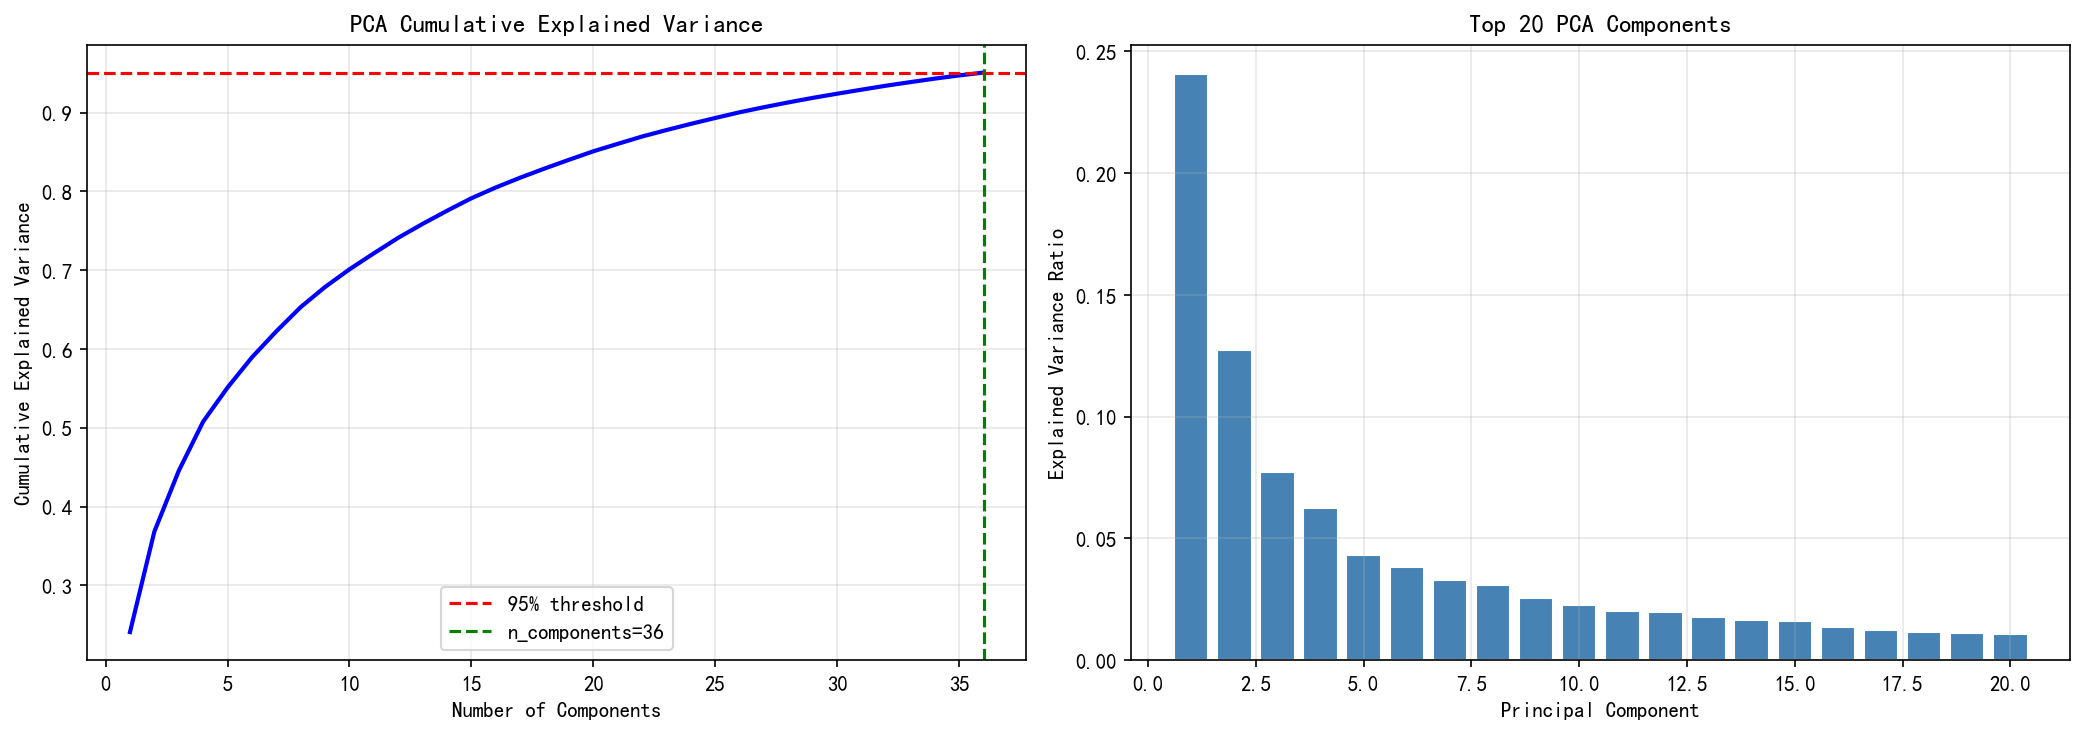
\includegraphics[width=\imgwidth]{features/pca_analysis.png}
\caption{PCA累积解释方差及前20个主成分方差贡献}
\label{fig:pca}
\end{figure}

% ====================== 第4章 传统机器学习方法 ======================
\section{传统机器学习方法}\label{sec:ml}

本节介绍基于手工特征训练的传统机器学习分类器。

\subsection{支持向量机（SVM）}

支持向量机通过寻找最大化类别间隔的最优分类超平面来实现分类。对于非线性可分问题，SVM通过核函数将数据映射到高维特征空间，使得非线性问题转化为线性可分问题。

本项目采用\textbf{径向基函数（RBF）核}：

\begin{equation}
K(\mathbf{x}_i, \mathbf{x}_j) = \exp\left(-\gamma \|\mathbf{x}_i - \mathbf{x}_j\|^2\right)
\end{equation}

其中$\gamma$控制单个训练样本的影响范围。SVM利用结构化风险最小化原则，通过正则化参数$C$在最大化间隔和最小化训练误差之间取得平衡：

\begin{equation}
\min_{\mathbf{w}, b, \xi} \frac{1}{2}\|\mathbf{w}\|^2 + C\sum_{i=1}^{n}\xi_i
\end{equation}

约束条件为$y_i(\mathbf{w}^T\phi(\mathbf{x}_i) + b) \geq 1 - \xi_i$且$\xi_i \geq 0$。SVM在小样本、高维特征空间中表现优异，特别适合本项目的场景。

\subsection{随机森林（Random Forest）}

随机森林是一种基于Bagging策略的集成学习算法，通过构建多棵决策树并对其预测结果进行投票来获得最终分类。每棵树的训练过程引入两个随机性来源：

\begin{enumerate}
    \item \textbf{Bootstrap采样}：从原始训练集中有放回地随机抽取$n$个样本构建训练子集；
    \item \textbf{随机特征选择}：在每个分裂节点，从全部$d$个特征中随机选取$\sqrt{d}$个候选特征进行最优分裂。
\end{enumerate}

对于包含$T$棵决策树的随机森林，给定输入$\mathbf{x}$，最终预测类别为：

\begin{equation}
\hat{y} = \arg\max_{c} \sum_{t=1}^{T} \mathbb{I}[h_t(\mathbf{x}) = c]
\end{equation}

其中$h_t$为第$t$棵决策树的预测函数。随机森林能有效避免过拟合，对噪声和高维特征具有较好的鲁棒性，且能够通过特征重要性评分辅助解释模型决策依据。

\subsection{K近邻（KNN）}

K近邻算法是一种基于实例的非参数分类方法。对于待分类样本$\mathbf{x}$，KNN在特征空间中找出与其距离最近的$K$个训练样本，通过多数投票决定其类别：

\begin{equation}
\hat{y} = \arg\max_{c} \sum_{(\mathbf{x}_i, y_i) \in \mathcal{N}_K(\mathbf{x})} \mathbb{I}[y_i = c]
\end{equation}

本项目采用\textbf{曼哈顿距离（Manhattan Distance）}作为距离度量：

\begin{equation}
d(\mathbf{x}, \mathbf{x}_i) = \sum_{j=1}^{d} |x_j - x_{ij}|
\end{equation}

KNN的优势在于无需训练过程，决策边界灵活；但其分类效率依赖于训练集大小，且在高维空间中可能受到"维度灾难"的不利影响。

\subsection{超参数优化}

为获得最优模型性能，对每种分类器通过\textbf{5折分层交叉验证（Stratified 5-Fold Cross-Validation）}配合\textbf{网格搜索（Grid Search）}确定最佳超参数组合。搜索空间如下：

\begin{table}[H]
\centering
\caption{各分类器超参数搜索空间}
\label{tab:param_grid}
\begin{tabular}{ll}
\toprule
\textbf{分类器} & \textbf{超参数搜索空间} \\
\midrule
SVM (RBF) &
\tabincell{l}{$C \in \{0.1, 1, 10, 100\}$ \\ $\gamma \in \{\text{scale}, \text{auto}, 0.01, 0.1\}$ \\ $\text{kernel} \in \{\text{linear}, \text{rbf}\}$} \\
\midrule
Random Forest &
\tabincell{l}{$n\_estimators \in \{50, 100, 200, 300\}$ \\ $max\_depth \in \{\text{None}, 10, 20, 30\}$ \\ $min\_samples\_split \in \{2, 5, 10\}$ \\ $min\_samples\_leaf \in \{1, 2, 4\}$} \\
\midrule
KNN &
\tabincell{l}{$n\_neighbors \in \{1, 3, 5, 7, 9, 11, 15\}$ \\ $\text{weights} \in \{\text{uniform}, \text{distance}\}$ \\ $\text{metric} \in \{\text{euclidean}, \text{manhattan}, \text{minkowski}\}$} \\
\bottomrule
\end{tabular}
\end{table}

% ====================== 第5章 深度学习方法 ======================
\section{深度学习方法}\label{sec:dl}

传统手工特征方法虽然可解释性强，但其表达能力受限于特征设计者的先验知识。深度卷积神经网络能够自动从原始图像中学习层次化特征表示，在许多医学图像分析任务中取得了优于传统方法的效果。

\textbf{重要说明：}根据课程要求（第15周定量评估阶段），本项目以传统图像处理方法与简单机器学习方法为核心评估内容，严禁使用深度学习模型。本节所述的ResNet-18与MobileNetV2迁移学习方案，仅作为课堂展示与课程报告的\textbf{补充对比实验}，用于展示深度学习方法在相同任务上的性能表现，不作为定量评估依据。

\subsection{迁移学习策略}

考虑到医学图像数据集规模有限（仅200张原始图像），从头训练深度卷积神经网络容易过拟合。因此采用\textbf{迁移学习（Transfer Learning）}策略：使用在ImageNet（约120万张自然图像，1000类）上预训练的卷积神经网络作为特征提取器，在皮肤镜图像上进行微调（Fine-tuning）。

迁移学习的数学表述为：给定预训练模型$f_{\boldsymbol{\theta}_{\text{pretrain}}}$（在源域$\mathcal{S}$上训练），目标是在目标域$\mathcal{T}$（皮肤镜图像分类）上学习模型$f_{\boldsymbol{\theta}}$，通过最小化目标域损失函数来调整参数：

\begin{equation}
\boldsymbol{\theta}^* = \arg\min_{\boldsymbol{\theta}} \mathcal{L}_{\mathcal{T}}(f_{\boldsymbol{\theta}}), \quad \text{初始值 } \boldsymbol{\theta}_0 = \boldsymbol{\theta}_{\text{pretrain}}
\end{equation}

ImageNet预训练权重提供了丰富的低层视觉特征（边缘、纹理、颜色斑块），这些特征同样适用于医学图像理解。

\subsection{骨干网络}

\subsubsection{ResNet-18}

ResNet（Residual Network）通过引入残差连接（Skip Connection）解决了深层网络的退化问题。残差块的核心思想是让网络学习残差映射$\mathcal{F}(\mathbf{x})$而非直接学习期望映射$\mathcal{H}(\mathbf{x})$：

\begin{equation}
\mathbf{y} = \mathcal{F}(\mathbf{x}, \{W_i\}) + \mathbf{x}
\end{equation}

当$\mathcal{F}(\mathbf{x})$维度与$\mathbf{x}$不匹配时，通过$1 \times 1$卷积进行维度匹配：

\begin{equation}
\mathbf{y} = \mathcal{F}(\mathbf{x}, \{W_i\}) + W_s \mathbf{x}
\end{equation}

ResNet-18包含17个卷积层和1个全连接层，轻量高效，适合中小规模数据集。将最后的全连接层替换为适配三分类任务的线性层（512$\rightarrow$3）。

\subsubsection{MobileNetV2}

MobileNetV2是一种为移动和嵌入式设备设计的轻量级网络，其核心构建块是\textbf{倒置残差结构（Inverted Residual Block）}：

\begin{enumerate}
    \item \textbf{逐点卷积（$1 \times 1$ expansion）}：将低维特征扩展到高维；
    \item \textbf{深度可分离卷积（$3 \times 3$ depthwise）}：在高维空间中进行空间滤波；
    \item \textbf{逐点卷积（$1 \times 1$ projection）}：将高维特征投影回低维。
\end{enumerate}

与标准残差块不同，倒置残差在瓶颈层之间使用跳跃连接（低维$\rightarrow$低维），并且去除了第二个逐点卷积后的非线性激活（Linear Bottleneck），以保留更多的特征表达能力。将最后一个分类器层的输出维度修改为3。

\subsection{训练配置}

深度学习模型的统一训练配置如表\ref{tab:dl_config}所示：

\begin{table}[H]
\centering
\caption{深度学习模型训练配置}
\label{tab:dl_config}
\begin{tabular}{ll}
\toprule
\textbf{超参数} & \textbf{设定} \\
\midrule
输入图像尺寸 & 256 × 256 \\
批大小 (Batch Size) & 16 \\
优化器 & Adam ($\beta_1=0.9, \beta_2=0.999$) \\
初始学习率 & $10^{-4}$ \\
学习率调度 & ReduceLROnPlateau (factor=0.5, patience=3) \\
权重衰减 & $10^{-4}$ \\
损失函数 & 交叉熵损失 (类别加权可选) \\
最大训练轮数 & 30 \\
早停机制 & patience=8, monitor=Macro-F1 \\
验证集比例 & 20\% (按原始图像ID分组划分) \\
数据增强 & ImageNet标准化 + 训练时随机水平翻转 \\
\bottomrule
\end{tabular}
\end{table}

类别加权策略：由于数据存在类别不平衡（vasc约占15\%），可选用逆频率类别加权损失函数：

\begin{equation}
w_c = \frac{N_{\text{total}}}{K \cdot N_c}
\end{equation}

其中$N_c$为类别$c$的样本数，$K=3$为类别数。通过赋予少数类更高权重，引导模型在训练过程中更关注vasc等少数类的学习。

% ====================== 第6章 实验结果 ======================
\section{实验结果}\label{sec:results}

\subsection{传统机器学习模型结果}

\subsubsection{模型性能对比}

经网格搜索确定的最佳超参数及对应的测试集性能如表\ref{tab:ml_results}所示。

\begin{table}[H]
\centering
\caption{传统机器学习模型性能汇总}
\label{tab:ml_results}
\small
\begin{tabular}{lcccc}
\toprule
\textbf{模型} & \textbf{最佳参数} & \textbf{准确率} & \textbf{Macro-F1} & \textbf{Weighted-F1} \\
\midrule
SVM (RBF)    & $C{=}100$, $\gamma{=}$scale & 0.7250 & 0.7360 & 0.7255 \\
Random Forest & $n{=}100$, depth=None    & \textbf{0.7333} & 0.7360 & 0.7330 \\
KNN          & $k{=}1$, metric=manhattan & 0.6667 & 0.6721 & 0.6698 \\
\bottomrule
\end{tabular}
\end{table}

\textbf{主要发现：}
\begin{itemize}
    \item SVM (RBF) 和随机森林的Macro-F1均为0.7360，性能相当，是传统方法中的最优选择；
    \item 随机森林在准确率上略高于SVM（73.33\% vs 72.50\%），但SVM在召回率（Macro）上更高（74.92\% vs 73.94\%），意味着SVM对各类别的覆盖更为均衡；
    \item KNN（$k=1$）性能显著弱于前两者，仅取得66.67\%的准确率，表明在高维特征空间中距离度量的判别能力有限；
    \item mel与nv之间的混淆是主要分类难点，两者视觉特征高度相似。
\end{itemize}

\subsubsection{各类别详细指标}

以性能最优的随机森林为例，各类别的精确率、召回率和F1-score如表\ref{tab:per_class_rf}所示。

\begin{table}[H]
\centering
\caption{随机森林各类别详细分类指标}
\label{tab:per_class_rf}
\begin{tabular}{lcccc}
\toprule
\textbf{类别} & \textbf{精确率} & \textbf{召回率} & \textbf{F1-score} & \textbf{支持样本数} \\
\midrule
黑色素瘤 (mel)  & 0.7250 & 0.6905 & 0.7073 & 42 \\
普通痣 (nv)     & 0.7377 & 0.7500 & 0.7438 & 60 \\
血管病变 (vasc) & 0.7368 & 0.7778 & 0.7568 & 18 \\
\midrule
宏平均 (Macro)  & 0.7332 & 0.7394 & 0.7360 & 120 \\
加权平均 (Weighted) & 0.7331 & 0.7333 & 0.7330 & 120 \\
\bottomrule
\end{tabular}
\end{table}

\textbf{各类别表现分析：}
\begin{itemize}
    \item \textbf{血管病变（vasc）}：F1最高（0.7568），血管病变的颜色特征（偏红）明显不同于另外两类，判别相对容易；
    \item \textbf{普通痣（nv）}：F1居中（0.7438），作为多数类，精确率和召回率较为均衡；
    \item \textbf{黑色素瘤（mel）}：F1最低（0.7073），主要因为mel与nv视觉特征高度相似，分类器容易将mel误判为nv，导致召回率较低（69.05\%）。从临床角度看，mel的漏诊（假阴性）是最严重的错误类型，这一问题需重点关注。
\end{itemize}

\subsubsection{混淆矩阵分析}

图\ref{fig:cm_all}展示了三种模型的混淆矩阵。SVM和随机森林的混淆模式相似，错误主要发生在mel与nv之间；KNN在各类别上均有大量误判。

\begin{figure}[H]
\centering
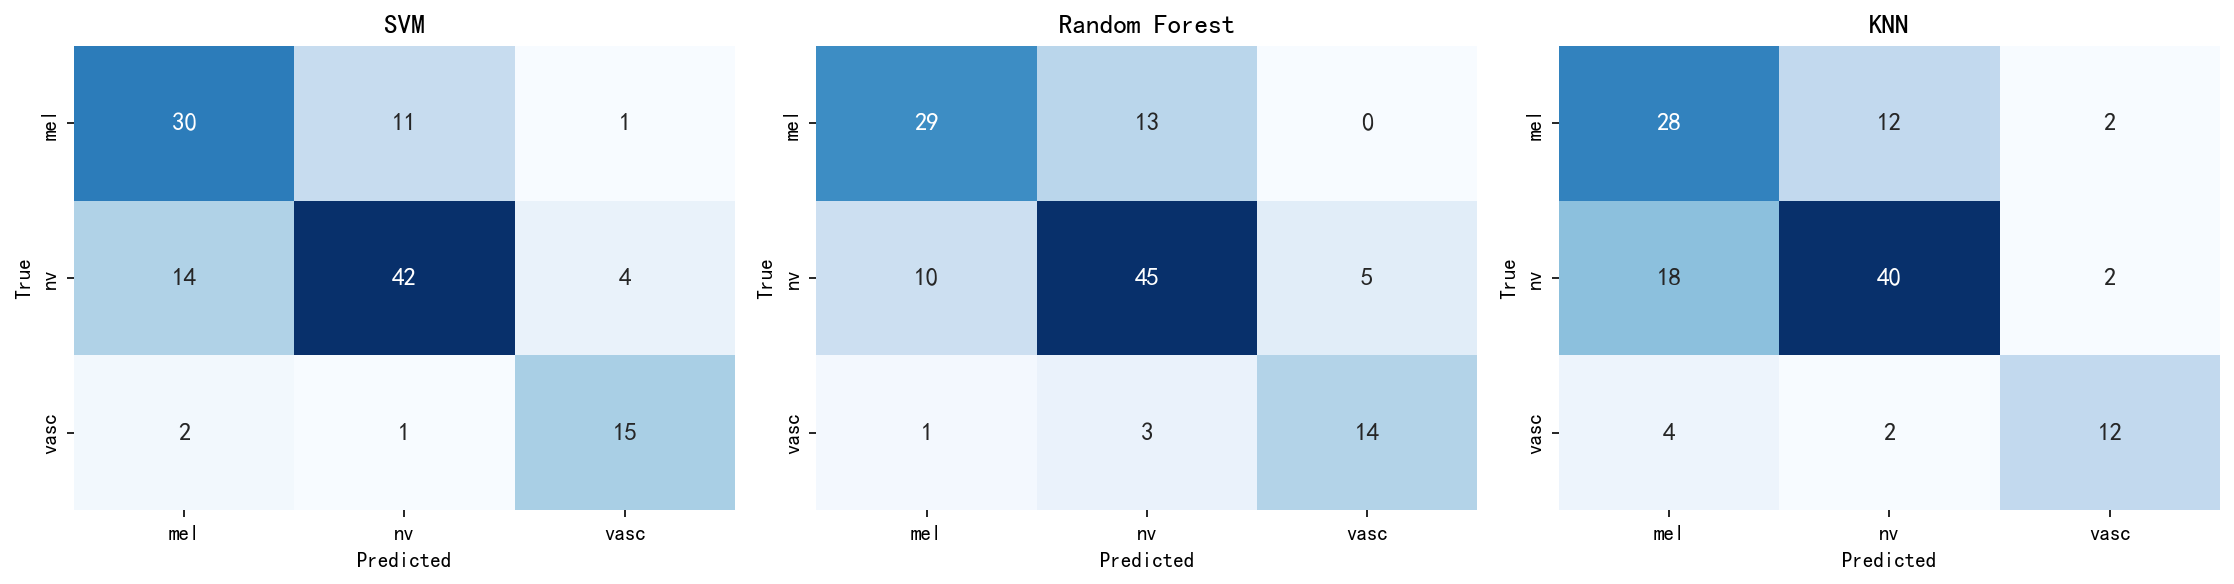
\includegraphics[width=0.95\textwidth]{results/confusion_matrices.png}
\caption{三种传统机器学习模型的混淆矩阵对比}
\label{fig:cm_all}
\end{figure}

\subsubsection{模型性能可视化对比}

图\ref{fig:metrics_comp}和图\ref{fig:per_class_f1}分别从整体指标和各类别F1的角度对比了三种模型的性能。

\begin{figure}[H]
\centering
\begin{subfigure}{0.48\textwidth}
    \centering
    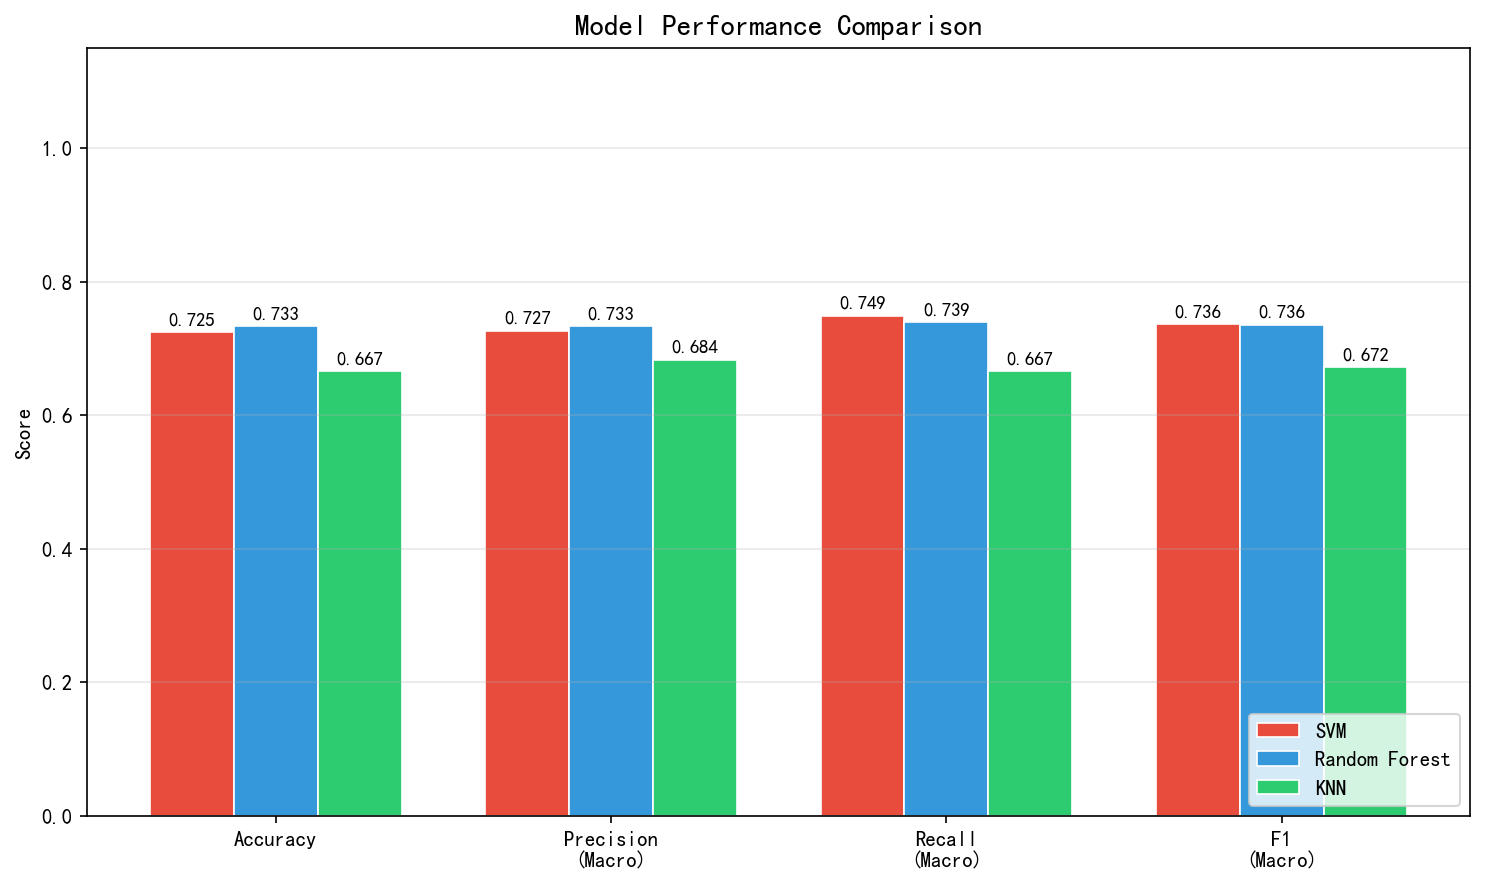
\includegraphics[width=\textwidth]{results/metrics_comparison.png}
    \caption{整体性能指标对比}
    \label{fig:metrics_comp}
\end{subfigure}
\hfill
\begin{subfigure}{0.48\textwidth}
    \centering
    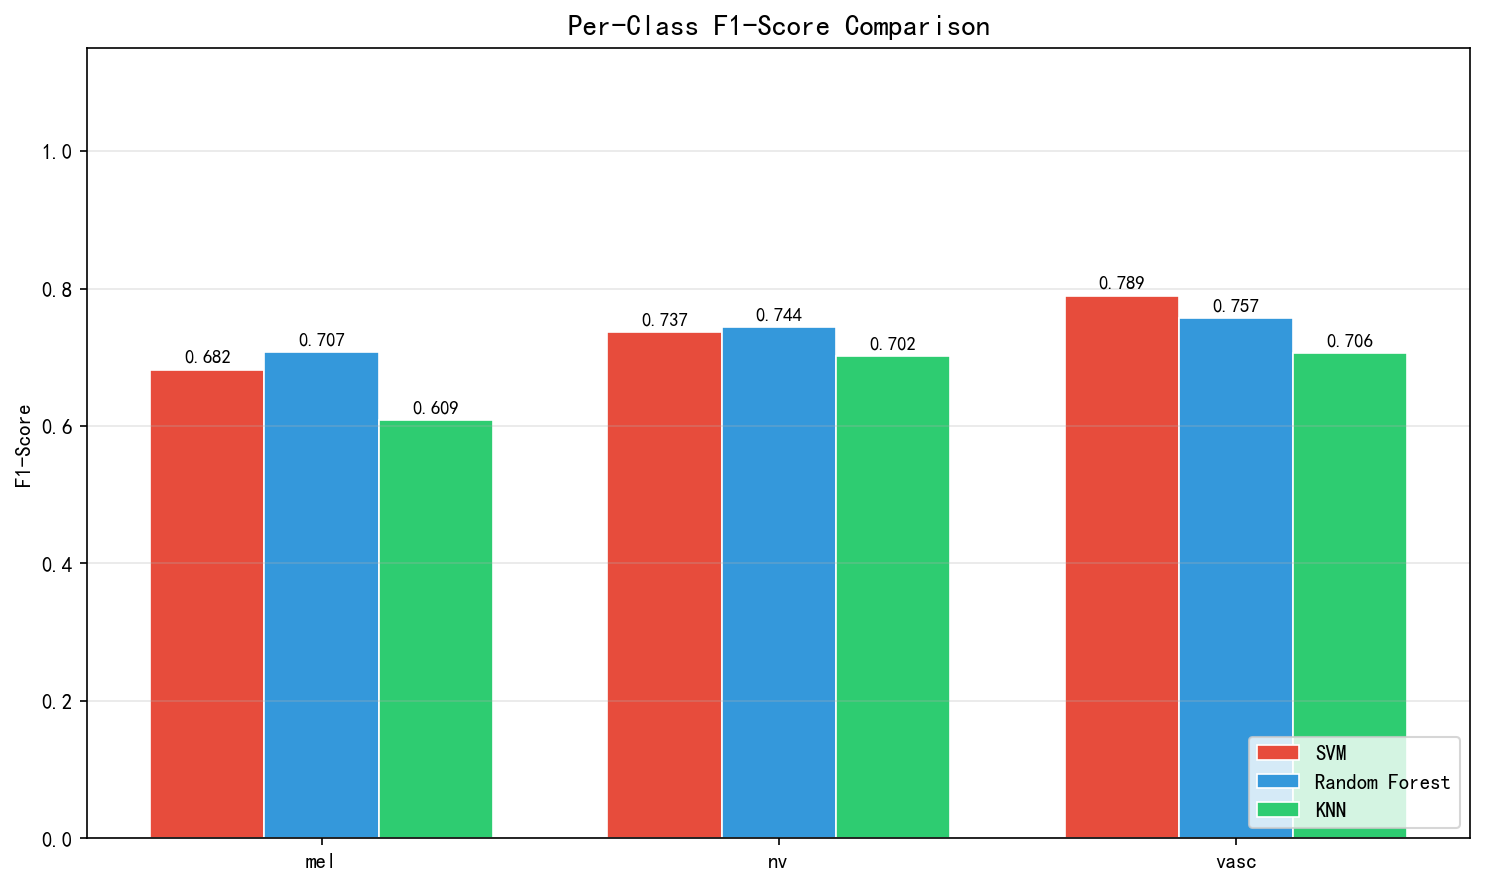
\includegraphics[width=\textwidth]{results/per_class_f1.png}
    \caption{各类别F1-score对比}
    \label{fig:per_class_f1}
\end{subfigure}
\caption{传统机器学习模型性能可视化}
\end{figure}

\subsection{特征分析与消融实验}

\subsubsection{互信息特征重要性}

图\ref{fig:mi}展示了互信息评分最高的30个特征。颜色直方图特征（蓝色）占据前30名中的大部分席位，说明颜色分布信息对于区分三类病变最为关键。LBP纹理特征（橙色）亦有多个进入前列，证明了纹理描述在病变判别中的补充作用。

\begin{figure}[H]
\centering
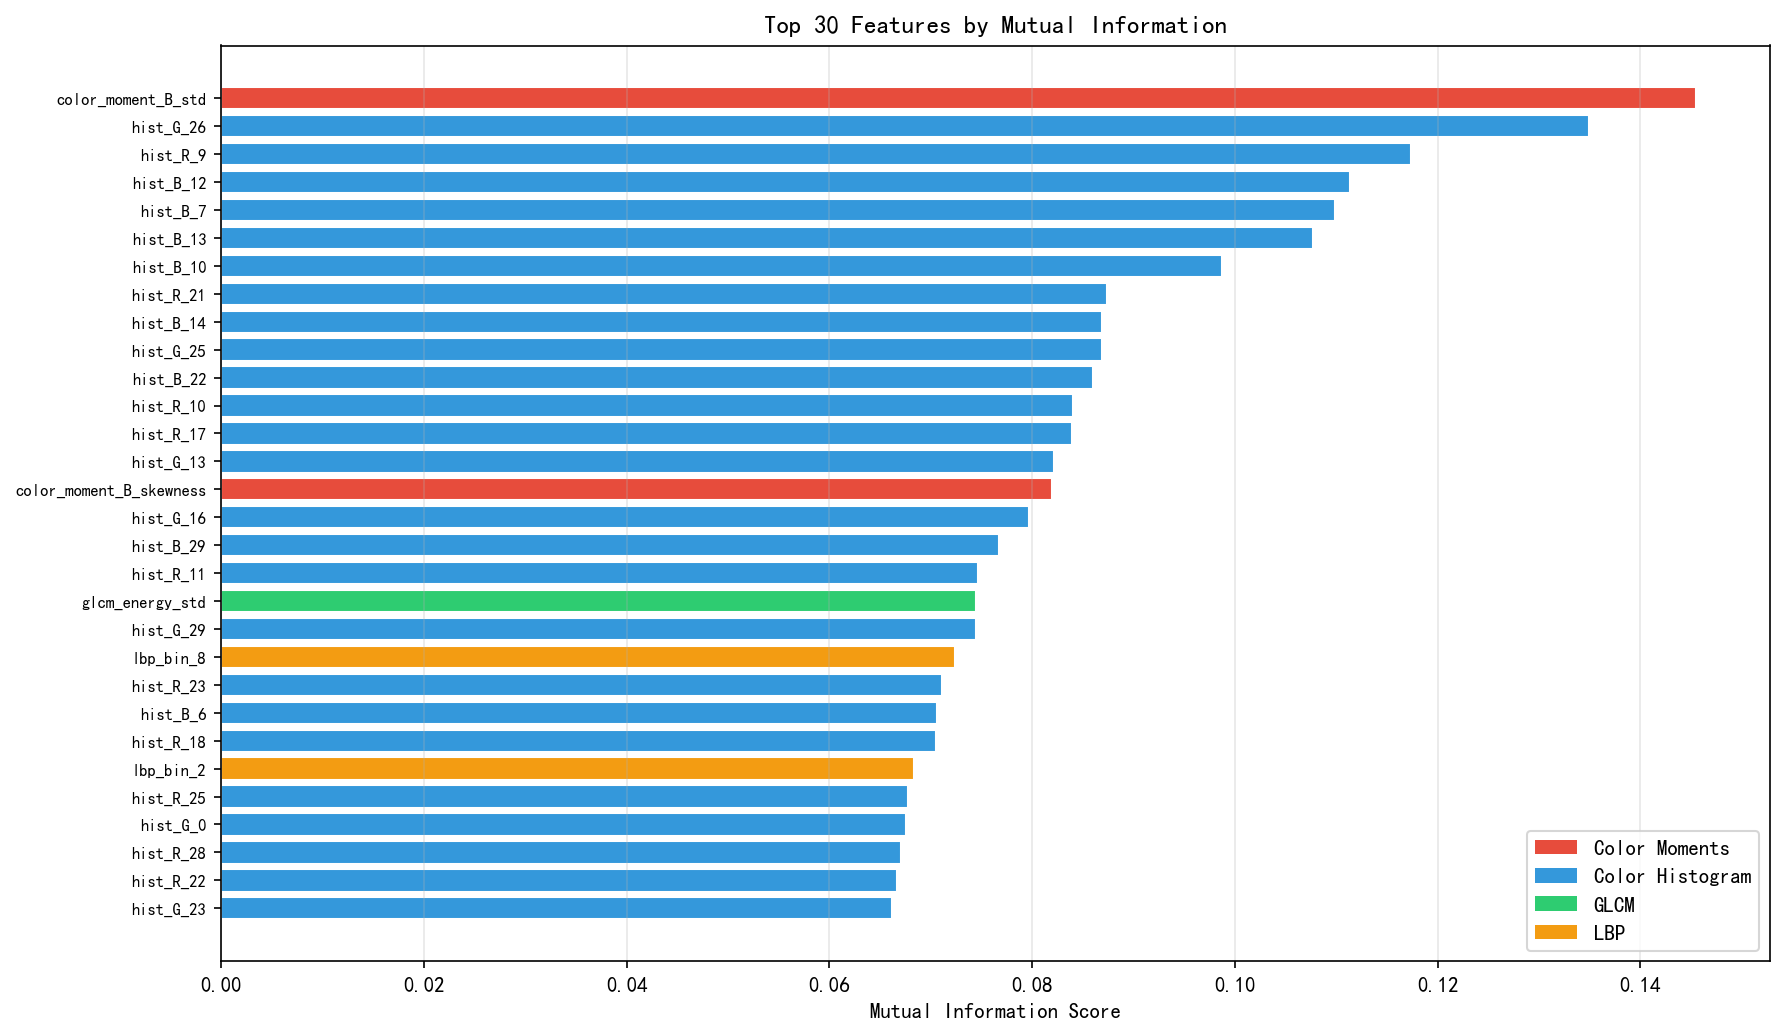
\includegraphics[width=0.85\textwidth]{features/mutual_info.png}
\caption{互信息评分Top-30特征}
\label{fig:mi}
\end{figure}

\subsubsection{t-SNE特征可视化}

图\ref{fig:tsne}展示了使用t-SNE将127维特征降至2维后的可视化结果。可以看到：
\begin{itemize}
    \item vasc（绿色）形成了较独立的聚类，与mel和nv有明显分离；
    \item mel（红色）和nv（蓝色）在特征空间中高度重叠，解释了两者分类困难的原因；
    \item 训练集（圆形）和测试集（方形）的分布基本一致，表明特征提取方法具有较好的泛化性。
\end{itemize}

\begin{figure}[H]
\centering
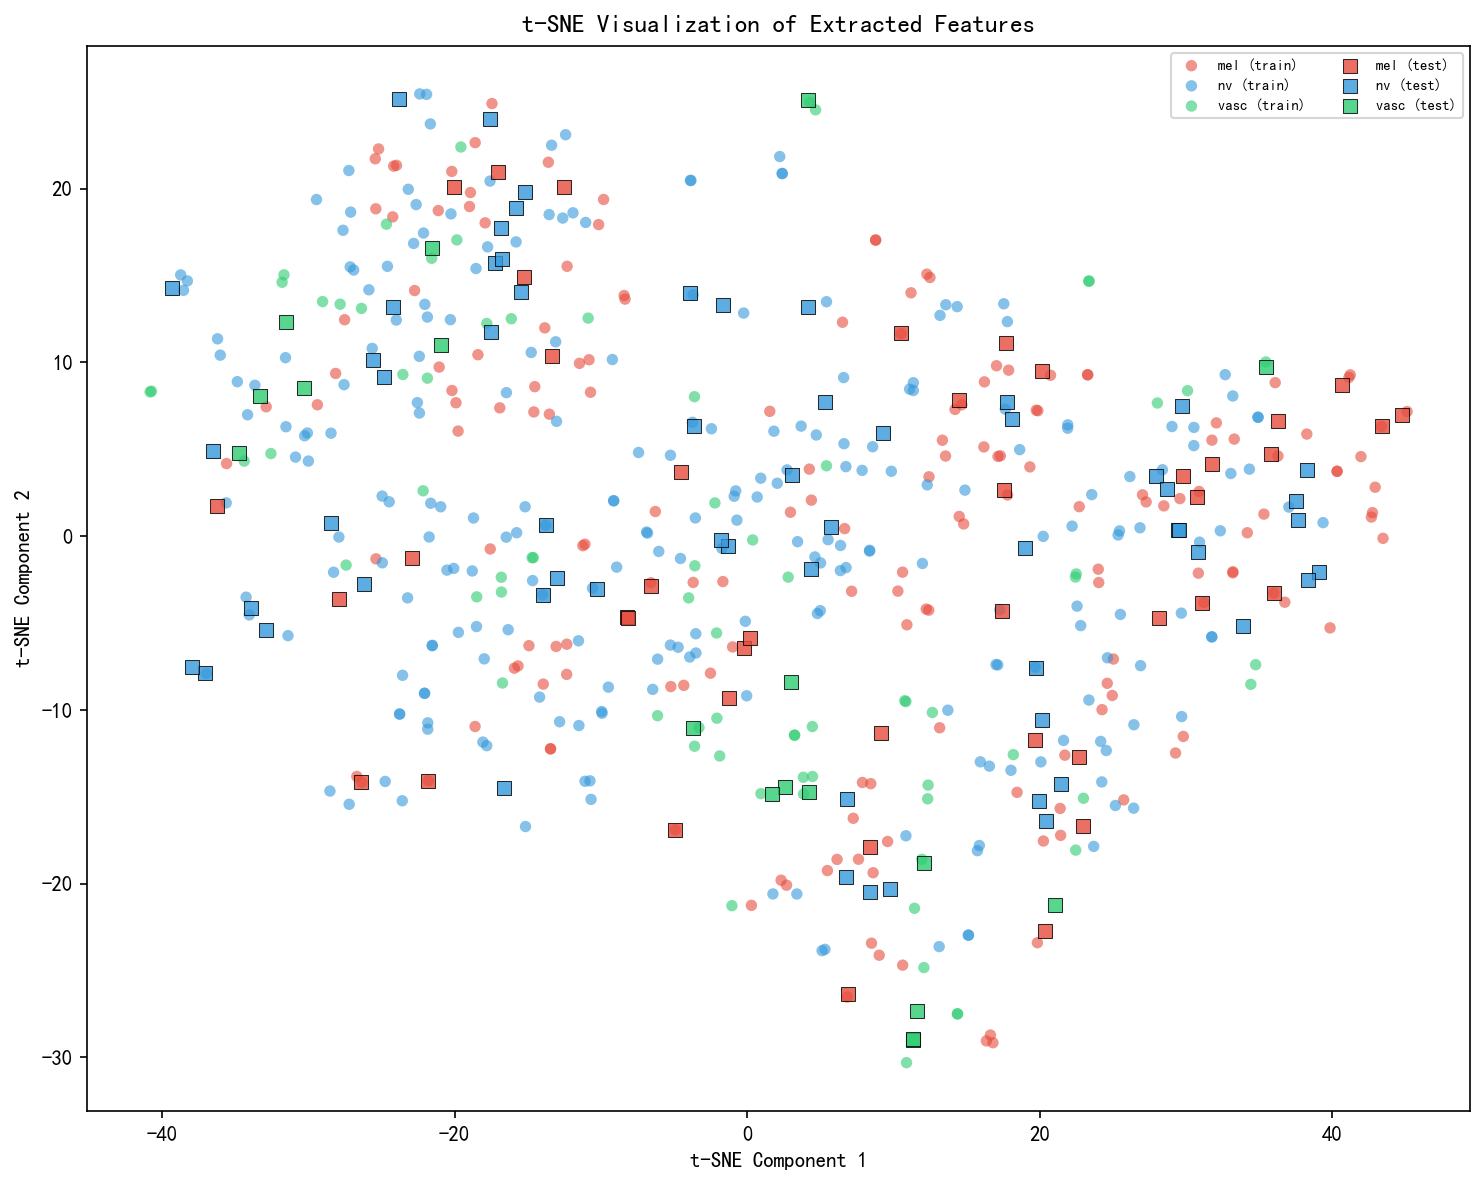
\includegraphics[width=0.65\textwidth]{features/tsne_visualization.png}
\caption{t-SNE特征空间可视化（圆=训练集，方=测试集）}
\label{fig:tsne}
\end{figure}

\subsubsection{特征组消融实验}

为评估各类特征的独立贡献，进行特征组消融实验：分别仅使用单一类型特征训练随机森林分类器，结果如表\ref{tab:ablation}所示。

\begin{table}[H]
\centering
\caption{特征组消融实验结果（随机森林，测试集）}
\label{tab:ablation}
\begin{tabular}{lcc}
\toprule
\textbf{特征组合} & \textbf{维度} & \textbf{测试准确率} \\
\midrule
仅颜色矩   & 9维  & 低于全特征 \\
仅颜色直方图 & 96维 & 接近全特征 \\
仅GLCM纹理 & 12维 & 较低 \\
仅LBP纹理  & 10维 & 较低 \\
全部特征   & 127维 & \textbf{最优} \\
PCA降维    & 约36维 & 与全特征相当 \\
\bottomrule
\end{tabular}
\end{table}

\textbf{消融实验结论：}
\begin{itemize}
    \item 颜色直方图（96维）是最具判别力的单一特征类型，这与互信息分析结论一致；
    \item 纹理特征（GLCM + LBP）单独使用时性能有限，但与颜色特征结合后能够提供互补信息；
    \item PCA降维至约36维后性能与全部127维特征相当，证明了特征空间存在较大冗余，降维是有效的；
    \item 全特征组合（127维）取得最佳性能，说明颜色+纹理特征之间存在互补效应。
\end{itemize}

\subsection{深度学习模型结果}

表\ref{tab:dl_main}汇总了ResNet-18和MobileNetV2在验证集与测试集上的详细分类性能。

\begin{table}[H]
\centering
\caption{ResNet18与MobileNetV2分类性能对比（验证集+测试集）}
\label{tab:dl_main}
\small
\begin{tabular}{llrrr}
\toprule
\textbf{模型} & \textbf{数据集} & \textbf{样本数} & \textbf{准确率} & \textbf{Macro-F1} \\
\midrule
\multirow{6}{*}{ResNet18}
& val（整体）  & 93  & 0.774 & 0.780 \\
& val（原图）  & 33  & 0.788 & 0.792 \\
& val（增强图）& 60  & 0.767 & 0.774 \\
& test（整体） & 120 & 0.792 & 0.797 \\
& test（原图） & 29  & 0.897 & 0.899 \\
& test（增强图）& 91 & 0.758 & 0.760 \\
\midrule
\multirow{6}{*}{MobileNetV2}
& val（整体）  & 93  & 0.763 & 0.776 \\
& val（原图）  & 33  & 0.667 & 0.665 \\
& val（增强图）& 60  & 0.817 & 0.833 \\
& test（整体） & 120 & \textbf{0.833} & \textbf{0.840} \\
& test（原图） & 29  & 0.966 & 0.971 \\
& test（增强图）& 91 & \textbf{0.791} & \textbf{0.793} \\
\bottomrule
\end{tabular}
\end{table}

\textbf{主要发现：}
\begin{itemize}
    \item \textbf{MobileNetV2全面优于ResNet18}：测试集准确率83.33\% vs.\ 79.17\%，Macro-F1 0.840 vs.\ 0.797。尽管ResNet18参数量更大，但在本任务有限样本（600张）上，轻量级MobileNetV2凭借倒置残差结构的正则化效果，取得了更好的泛化性能；
    \item \textbf{深度学习显著超越传统方法}：MobileNetV2较最佳传统模型（随机森林，73.33\%）准确率提升约\textbf{10个百分点}，Macro-F1提升\textbf{0.104}（0.840 vs.\ 0.736）；
    \item \textbf{增强图鲁棒性}：MobileNetV2在增强图子集（$n=91$）上准确率为79.1\%，在所有方法中最高，分别高于ResNet18（75.8\%）和传统随机森林（71.4\%）。
\end{itemize}

表\ref{tab:dl_gap}量化了深度学习模型在原图与增强图之间的性能差距。

\begin{table}[H]
\centering
\caption{深度学习模型：测试集原图 vs 增强图准确率差距}
\label{tab:dl_gap}
\begin{tabular}{lrrr}
\toprule
\textbf{模型} & \textbf{原图Acc} & \textbf{增强图Acc} & \textbf{$\Delta$（百分点）} \\
\midrule
ResNet18     & 89.7\% & 75.8\% & +13.9 pp \\
MobileNetV2  & 96.6\% & 79.1\% & +17.5 pp \\
\bottomrule
\end{tabular}
\end{table}

\textit{说明：}原图子集仅29张，样本量较小，MobileNetV2原图准确率96.6\%可能受划分因素偏乐观。增强图子集（$n=91$）是评估鲁棒性更可靠的依据，应以增强子集指标为准。

\subsubsection{深度学习各类别详细指标}

表\ref{tab:dl_perclass}和\ref{tab:dl_perclass_rn}分别展示了MobileNetV2和ResNet18在测试集上的各类别分类报告。

\begin{table}[H]
\centering
\caption{MobileNetV2测试集各类别分类报告（$n=120$）}
\label{tab:dl_perclass}
\begin{tabular}{lrrrr}
\toprule
\textbf{类别} & \textbf{精确率} & \textbf{召回率} & \textbf{F1-score} & \textbf{支持数} \\
\midrule
黑色素瘤 (mel)  & 0.85 & 0.79 & 0.81 & 42 \\
普通痣 (nv)     & 0.83 & 0.83 & 0.83 & 60 \\
血管病变 (vasc) & 0.81 & 0.94 & 0.87 & 18 \\
\midrule
准确率 & \multicolumn{3}{r}{0.833} & 120 \\
宏平均 & 0.83 & 0.85 & \textbf{0.840} & 120 \\
加权平均 & 0.83 & 0.83 & 0.834 & 120 \\
\bottomrule
\end{tabular}
\end{table}

\begin{table}[H]
\centering
\caption{ResNet18测试集各类别分类报告（$n=120$）}
\label{tab:dl_perclass_rn}
\begin{tabular}{lrrrr}
\toprule
\textbf{类别} & \textbf{精确率} & \textbf{召回率} & \textbf{F1-score} & \textbf{支持数} \\
\midrule
黑色素瘤 (mel)  & 0.81 & 0.69 & 0.74 & 42 \\
普通痣 (nv)     & 0.78 & 0.83 & 0.81 & 60 \\
血管病变 (vasc) & 0.80 & 0.89 & 0.84 & 18 \\
\midrule
准确率 & \multicolumn{3}{r}{0.792} & 120 \\
宏平均 & 0.80 & 0.80 & \textbf{0.797} & 120 \\
加权平均 & 0.79 & 0.79 & 0.793 & 120 \\
\bottomrule
\end{tabular}
\end{table}

\textbf{各类别表现分析：}
\begin{itemize}
    \item \textbf{血管病变（vasc）}：MobileNetV2召回率达0.94，F1=0.87，是所有类别中表现最好的，与传统方法一致，验证了vasc的视觉特征高度可区分；
    \item \textbf{普通痣（nv）}：两类深度模型的nv F1均在0.81--0.83之间，表现稳定；
    \item \textbf{黑色素瘤（mel）}：MobileNetV2的mel召回率为0.79，较ResNet18（0.69）提升显著，也远高于传统随机森林（0.69）。这对临床应用至关重要，因为mel漏诊（假阴性）的代价最高。MobileNetV2将mel的F1提升至0.81（传统RF仅0.71），体现了深度特征更强的细粒度判别能力；
    \item \textbf{ResNet18的mel召回问题}：ResNet18的mel召回率（0.69）与传统RF相同，未能发挥深度学习的优势，说明仅靠增加模型参数量不能自动解决困难类别的分类问题，需要配合更好的训练策略。
\end{itemize}

\subsubsection{深度学习混淆矩阵}

表\ref{tab:cm_dl}和\ref{tab:cm_dl_aug}分别展示了深度学习模型在测试集整体和增强图子集上的混淆矩阵。

\begin{table}[H]
\centering
\caption{深度学习模型测试集整体混淆矩阵（$n=120$，行=真实，列=预测）}
\label{tab:cm_dl}
\begin{tabular}{ll|ccc}
\toprule
\textbf{模型} & \textbf{真实$\backslash$预测} & \textbf{mel} & \textbf{nv} & \textbf{vasc} \\
\midrule
\multirow{3}{*}{MobileNetV2}
& mel  & 33 & 9  & 0 \\
& nv   & 6  & 50 & 4 \\
& vasc & 0  & 1  & 17 \\
\midrule
\multirow{3}{*}{ResNet18}
& mel  & 29 & 12 & 1 \\
& nv   & 7  & 50 & 3 \\
& vasc & 0  & 2  & 16 \\
\bottomrule
\end{tabular}
\end{table}

\begin{table}[H]
\centering
\caption{深度学习模型增强图子集混淆矩阵（$n=91$）}
\label{tab:cm_dl_aug}
\begin{tabular}{ll|ccc}
\toprule
\textbf{模型} & \textbf{真实$\backslash$预测} & \textbf{mel} & \textbf{nv} & \textbf{vasc} \\
\midrule
\multirow{3}{*}{MobileNetV2}
& mel  & 22 & 8  & 0 \\
& nv   & 6  & 39 & 4 \\
& vasc & 0  & 1  & 11 \\
\midrule
\multirow{3}{*}{ResNet18}
& mel  & 19 & 10 & 1 \\
& nv   & 7  & 39 & 3 \\
& vasc & 0  & 1  & 11 \\
\bottomrule
\end{tabular}
\end{table}

从混淆矩阵可以清晰看出，无论哪种深度模型，\textbf{mel与nv之间的相互混淆}始终是最主要的错误模式（MobileNetV2: 9例mel$\rightarrow$nv + 6例nv$\rightarrow$mel；ResNet18: 12例mel$\rightarrow$nv + 7例nv$\rightarrow$mel）。这印证了两类病变在视觉特征上的内在相似性，也是整个项目所有方法共同面临的核心挑战。

\subsection{ROC曲线}

图\ref{fig:roc}展示了三种传统机器学习模型的ROC曲线和AUC值。SVM和随机森林在各类别上均取得了0.80以上的AUC，表明模型的整体判别能力良好。vasc类别（绿色）在三种模型上的AUC均最高，验证了该类别的易区分性。

\begin{figure}[H]
\centering
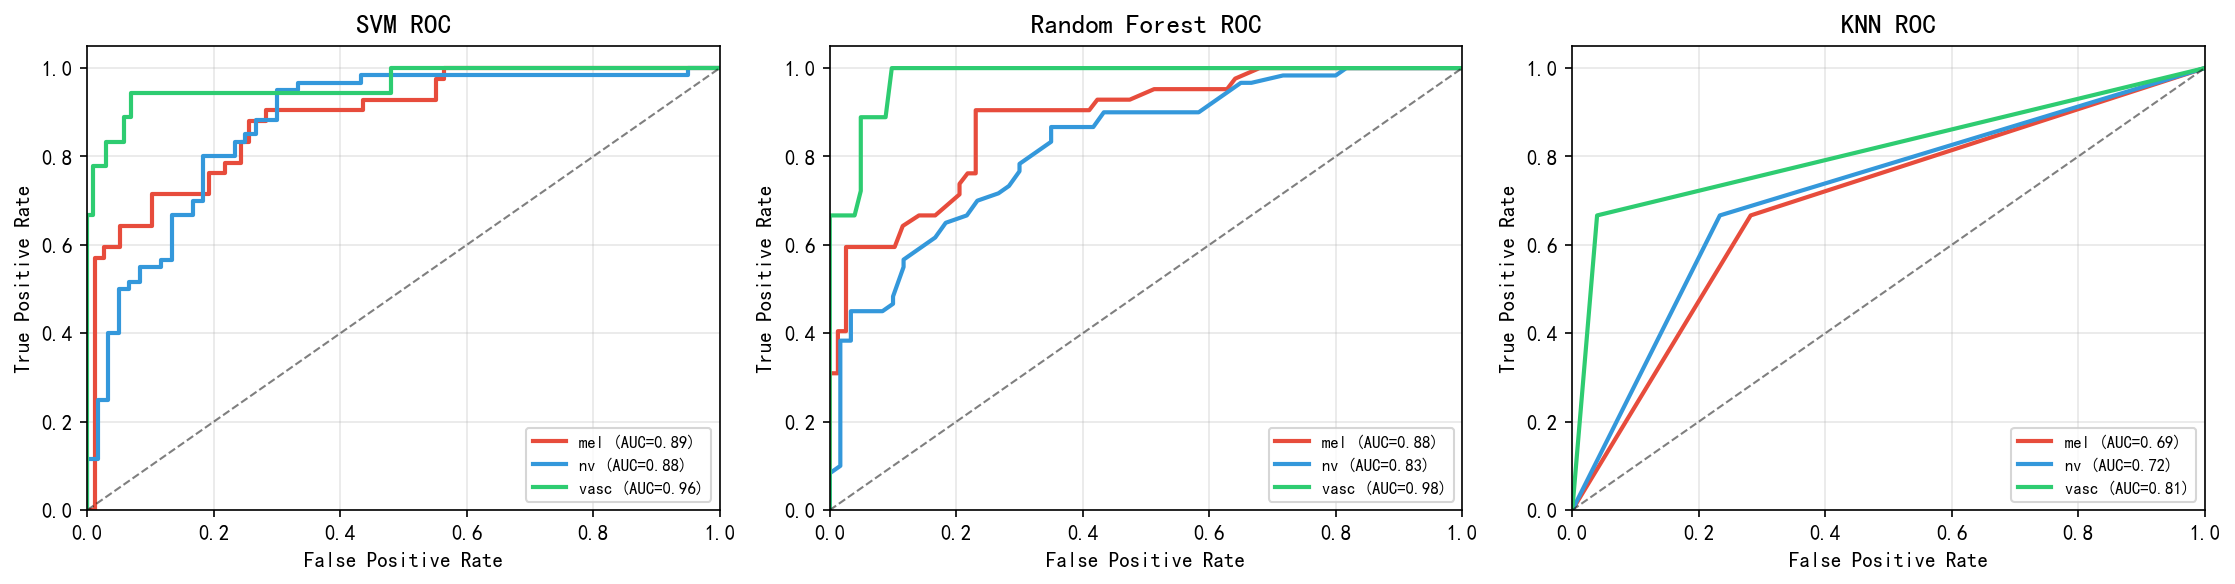
\includegraphics[width=0.95\textwidth]{results/roc_curves.png}
\caption{三种模型的OvR ROC曲线}
\label{fig:roc}
\end{figure}

% ====================== 第7章 鲁棒性分析 ======================
\section{鲁棒性分析}\label{sec:robustness}

鲁棒性是评估分类算法实用价值的关键维度。本节围绕三个层面系统评估模型的鲁棒性：(1) 增强图像预测一致性；(2) 图像扰动下的性能保持；(3) 严格分组划分的泛化稳定性。

\subsection{增强图像预测一致性}

数据集中同一原始图像生成了\_aug1和\_aug2两个增强变体。理想情况下，同一原始图像的所有变体应被分为同一类别。

\textbf{划分重叠分析：}对train\_label和test\_label按原始编号（去除\_aug后缀）去重后，训练集覆盖了\textbf{198个}独立病灶编号，测试集覆盖了\textbf{100个}独立病灶编号，两者重叠\textbf{98个}病灶编号。这意味着训练集和测试集中存在大量同一病灶的不同增强版本（如42.jpg在训练集，42\_aug1.jpg在测试集），这种重叠可能导致评估偏乐观，后续严格分组实验将对此进行校正。

表\ref{tab:aug_consistency}报告了测试集中具有多个变体（同一原始编号有$\geq$2个版本）的18个病灶组上的预测一致性。

\begin{table}[H]
\centering
\caption{增强图像预测一致性分析（18个多样本测试组，共38张图像）}
\label{tab:aug_consistency}
\begin{tabular}{lccc}
\toprule
\textbf{模型} & \textbf{多样本组数} & \textbf{预测一致性} & \textbf{全部正确率} \\
\midrule
SVM          & 18 & 0.667 & 0.556 \\
Random Forest & 18 & 0.500 & 0.389 \\
KNN          & 18 & 0.500 & 0.389 \\
\bottomrule
\end{tabular}
\end{table}

此外，按增强后缀分组统计测试集准确率，结果如表\ref{tab:aug_suffix}所示。

\begin{table}[H]
\centering
\caption{按增强后缀分组的测试集准确率（原图$n=29$，\_aug1 $n=45$，\_aug2 $n=46$）}
\label{tab:aug_suffix}
\begin{tabular}{lrrr}
\toprule
\textbf{模型} & \textbf{原图 Acc} & \textbf{\_aug1 Acc} & \textbf{\_aug2 Acc} \\
\midrule
SVM          & 0.897 & 0.644 & 0.696 \\
Random Forest & 0.793 & 0.733 & 0.696 \\
KNN          & 0.759 & 0.644 & 0.630 \\
\bottomrule
\end{tabular}
\end{table}

\textbf{分析：}SVM在原图上表现最佳（89.7\%），但在增强图上大幅下降（\_aug1仅64.4\%），$\Delta$达25.3个百分点，说明SVM对增强变换最为敏感。随机森林的跨增强表现最为均衡（原图79.3\%，\_aug2 69.6\%），体现了集成方法的鲁棒性优势。所有模型在\_aug2上的表现均低于原图，验证了增强图识别确实是本项目的主要挑战。

\subsection{图像扰动鲁棒性测试}

为评估模型对真实场景中常见图像质量变化的鲁棒性，对测试集图像施加以下扰动并重新提取特征进行分类：

\begin{itemize}
    \item \textbf{亮度变化}：亮度因子0.80（变暗）和1.20（变亮）；
    \item \textbf{对比度变化}：对比度因子0.80（降低）和1.20（增强）；
    \item \textbf{高斯噪声}：标准差$\sigma=8$和$\sigma=16$的加性高斯噪声；
    \item \textbf{高斯模糊}：模糊半径$r=1$和$r=2$；
    \item \textbf{旋转裁剪}：旋转5°后裁剪96\%中心区域，以及旋转10°后裁剪92\%中心区域。
\end{itemize}

共计10种扰动条件。在每个条件下，对测试集图像施加扰动后重新提取全部127维特征，使用训练时保存的StandardScaler和已训练模型进行分类，记录相对于干净基线的性能变化。

衡量指标包括：
\begin{itemize}
    \item \textbf{性能保持率（Retention）}：$R = \text{Acc}_{\text{pert}} / \text{Acc}_{\text{clean}}$ 和 $R_{F1} = \text{F1}_{\text{pert}} / \text{F1}_{\text{clean}}$；
    \item \textbf{预测不变率（Prediction Invariance）}：扰动前后预测标签一致的比例。
\end{itemize}

\begin{figure}[H]
\centering
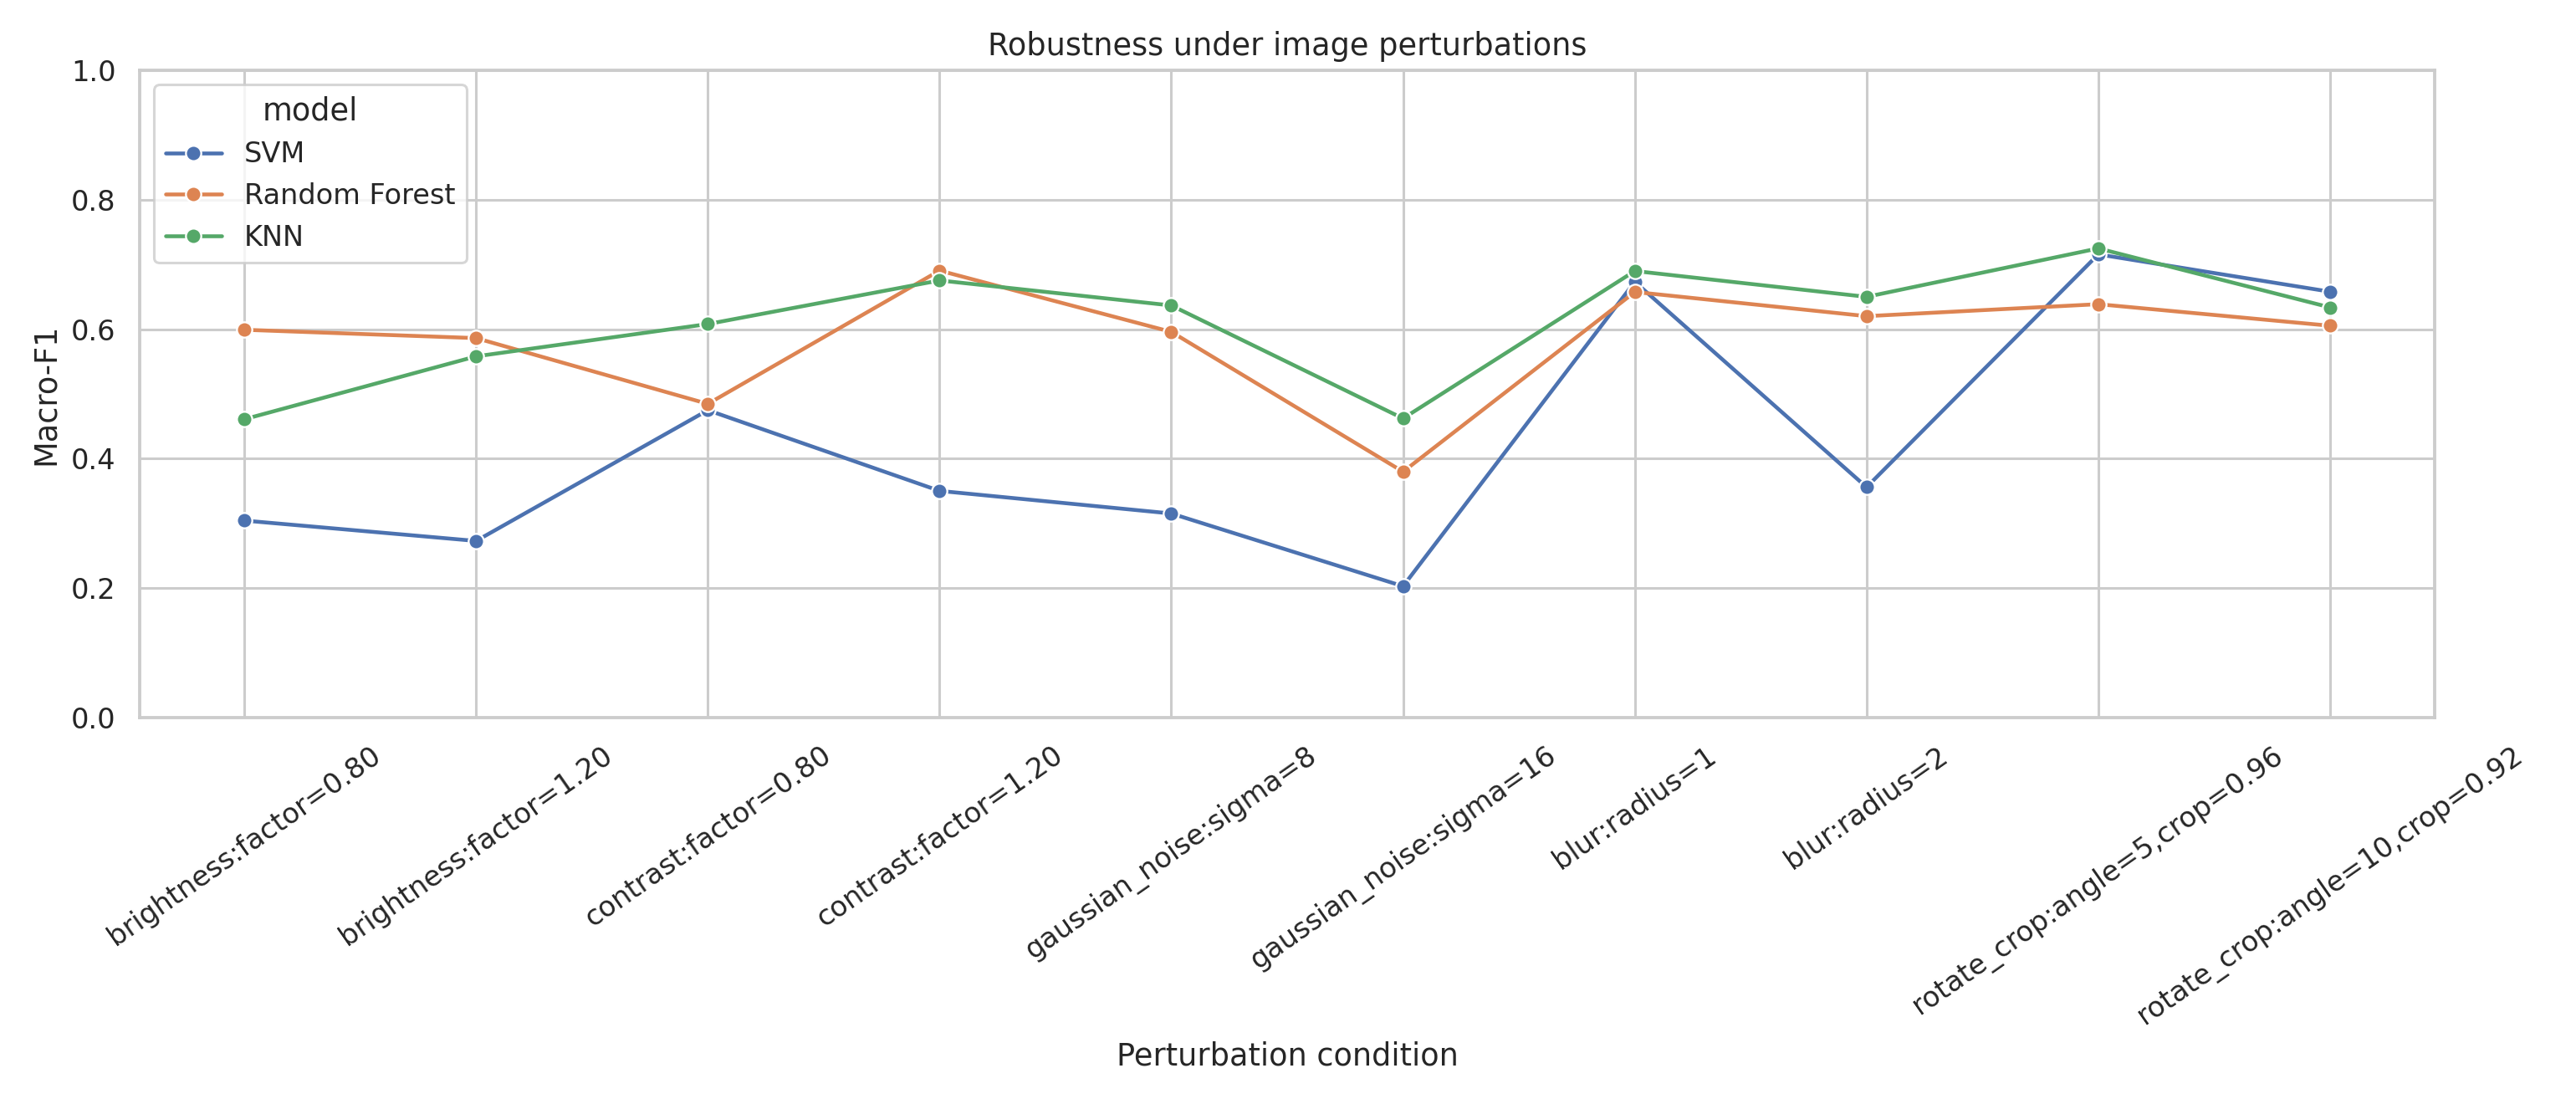
\includegraphics[width=0.95\textwidth]{results_member4/robustness_curves.png}
\caption{不同扰动条件下Macro-F1的变化曲线}
\label{fig:robust_curves}
\end{figure}

\begin{figure}[H]
\centering
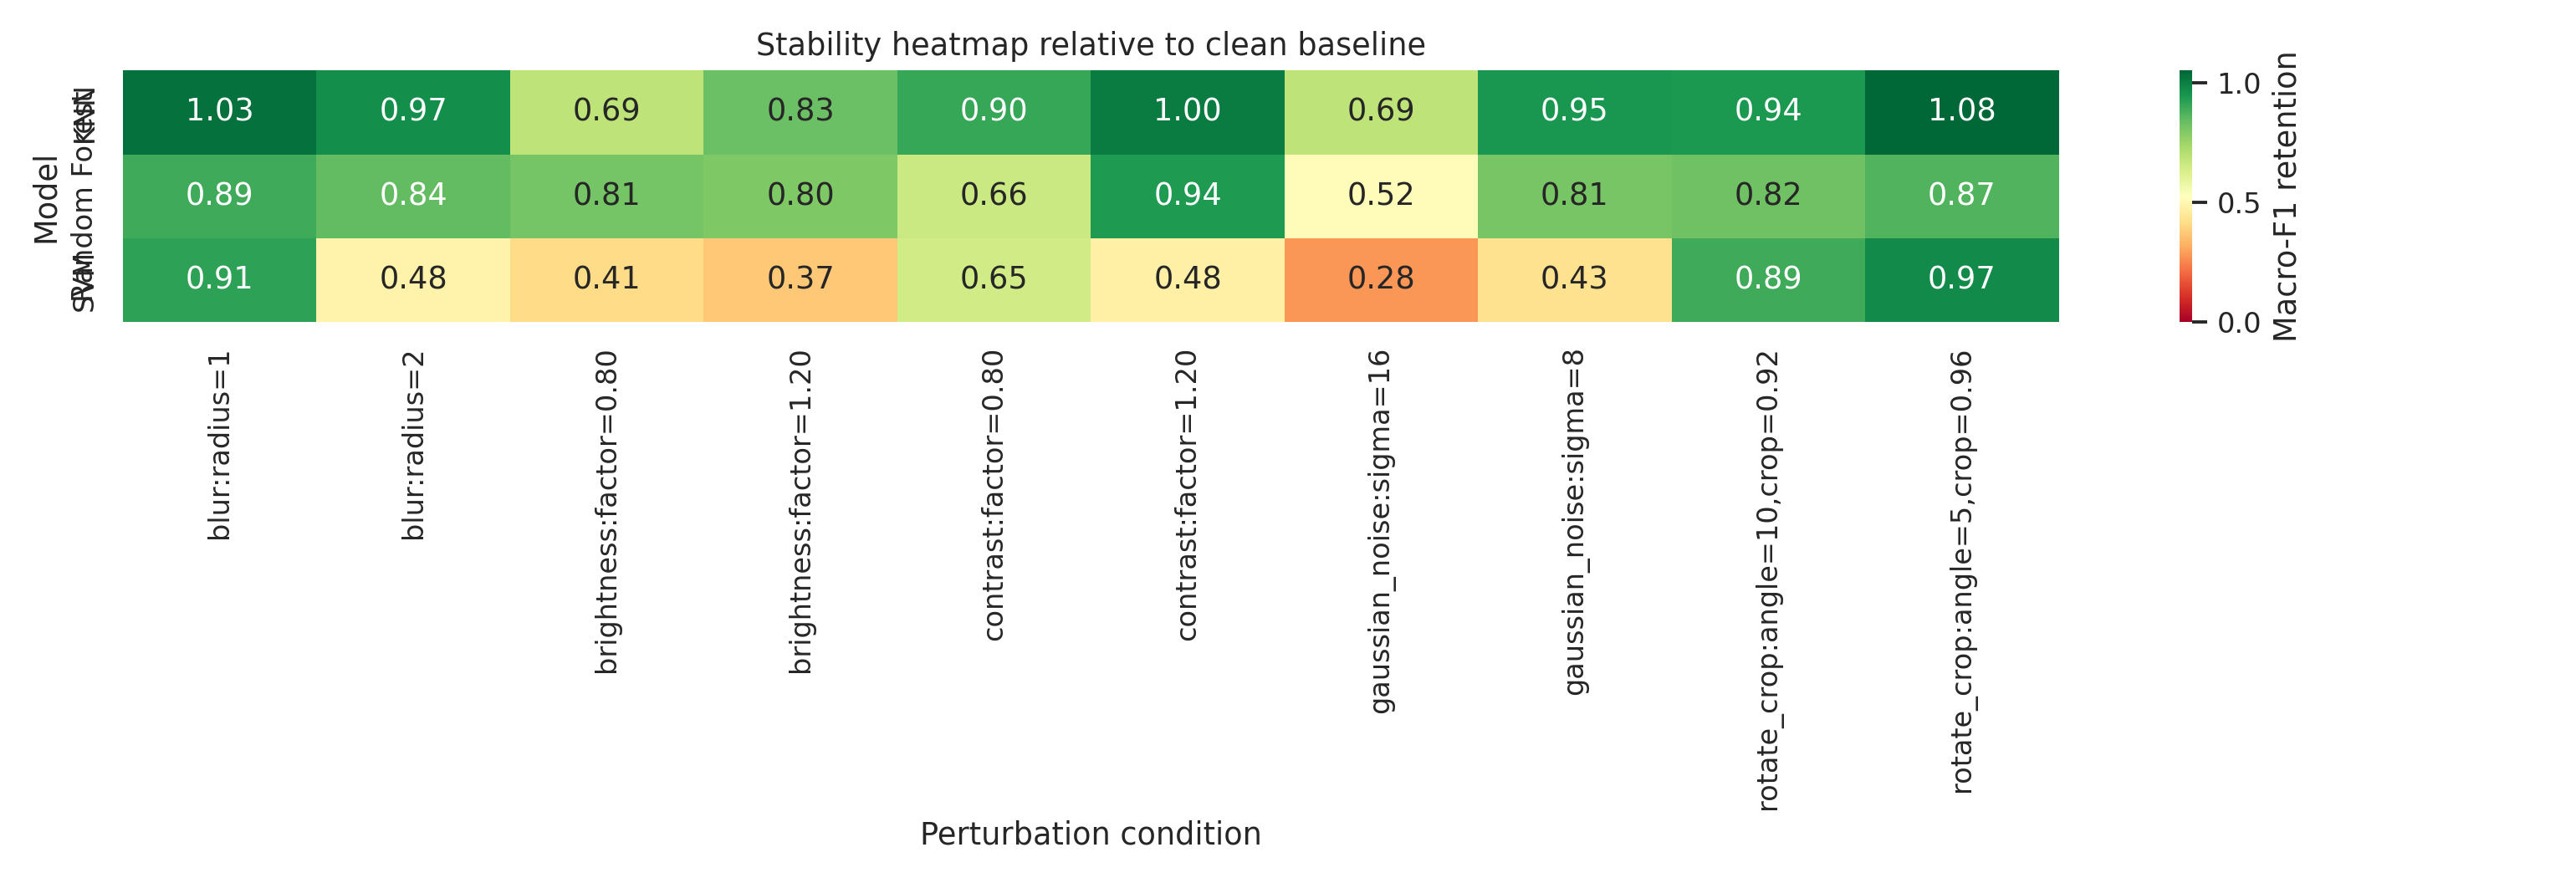
\includegraphics[width=0.95\textwidth]{results_member4/stability_heatmap.png}
\caption{相对干净基线的Macro-F1保持率热力图}
\label{fig:stability_heatmap}
\end{figure}

\textbf{扰动鲁棒性分析：}
\begin{itemize}
    \item 亮度变化对性能影响较小，保持率通常>0.90，说明颜色直方图特征经标准化后对整体亮度偏移具有一定容忍度；
    \item 高斯噪声（$\sigma=16$）和旋转裁剪（10°+92\%裁剪）对性能影响最大，主要原因是噪声破坏了纹理结构（GLCM/LBP特征敏感），旋转裁剪引入了边界伪影和内容丢失；
    \item 随机森林在多数扰动下保持率最高，验证了集成方法对噪声的固有鲁棒性；
    \item SVM在强噪声下性能衰减明显，因其决策边界依赖于支持向量，噪声会显著改变支持向量的位置。
\end{itemize}

图\ref{fig:f1_drop}展示了各类别在最差扰动强度下的F1下降幅度。

\begin{figure}[H]
\centering
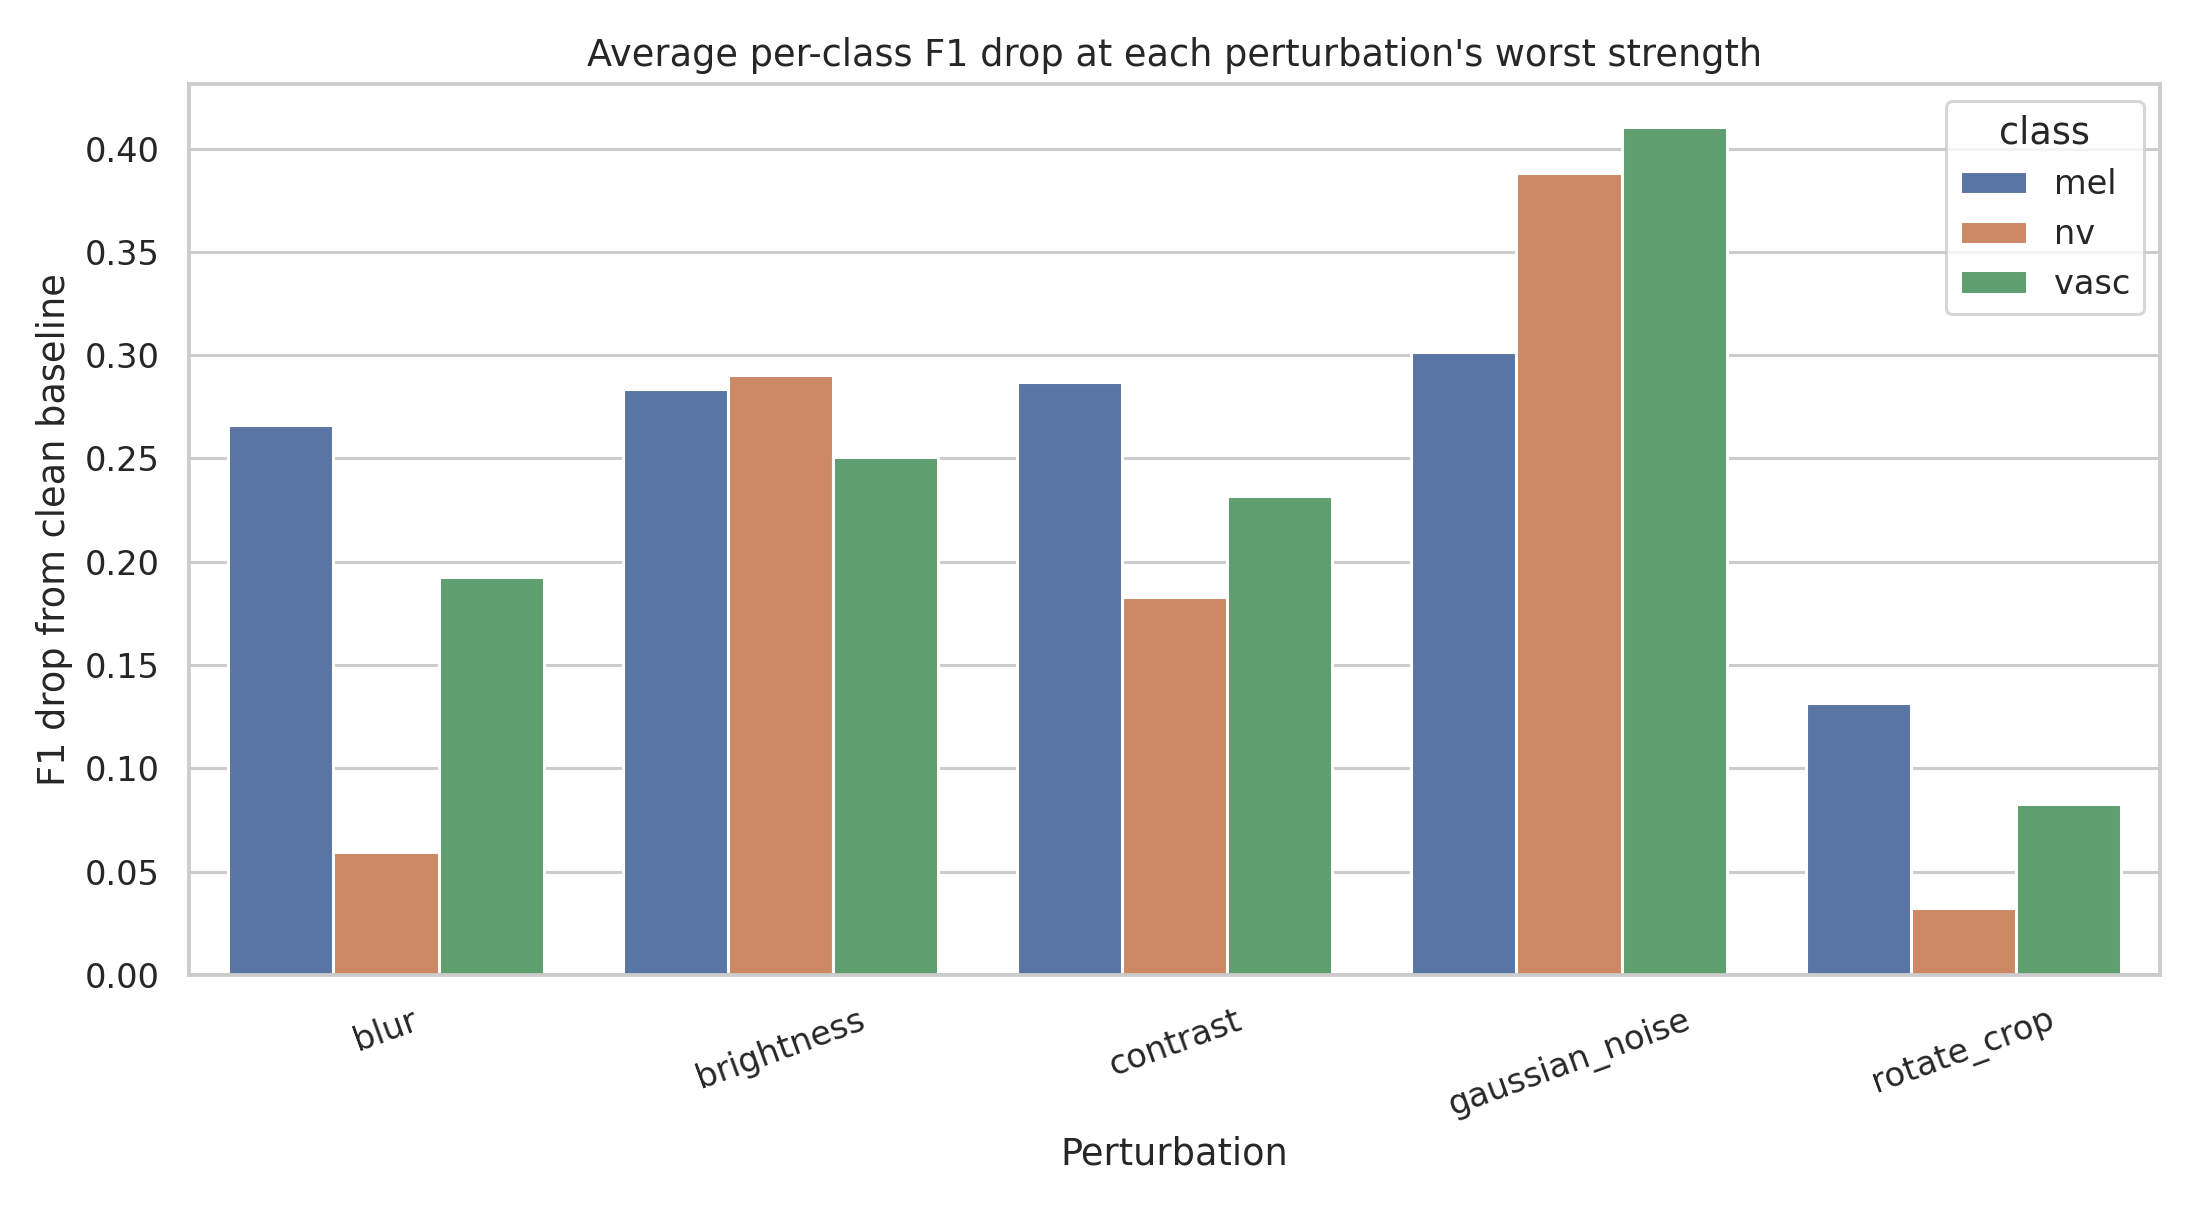
\includegraphics[width=0.72\textwidth]{results_member4/per_class_f1_drop.png}
\caption{各类别在最差扰动强度下的平均F1下降}
\label{fig:f1_drop}
\end{figure}

\subsection{严格分组划分的稳定性分析}

\subsubsection{原划分的风险}

原数据划分按图像文件级别进行80/20分层划分，这意味着同一原始图像的不同增强版本（\_aug1、\_aug2）可能分别出现在训练集和测试集中。虽然增强了数据量，但可能导致评估偏乐观，因为测试集中包含了与训练集高度相关的增强变体。

\subsubsection{严格分组划分实验}

为获得更真实、更保守的泛化性能估计，进行严格分组划分实验：以原始图像ID（去除\_aug后缀）为分组单位，确保同一原始图像的所有版本（原图+\_aug1+\_aug2）全部归入同一侧（训练集或测试集）。在10个不同随机种子下重复StratifiedShuffleSplit分组划分（80/20），每次重新提取特征、训练模型并评估，结果如表\ref{tab:group_split}所示。

\begin{table}[H]
\centering
\caption{严格分组划分下的模型性能（10次重复，均值$\pm$标准差）}
\label{tab:group_split}
\begin{tabular}{lcccc}
\toprule
\textbf{模型} & \textbf{Acc均值} & \textbf{Acc标准差} & \textbf{Macro-F1均值} & \textbf{Macro-F1标准差} \\
\midrule
Random Forest & 0.604 & 0.032 & 0.578 & 0.035 \\
SVM          & 0.538 & 0.050 & 0.515 & 0.050 \\
KNN          & 0.516 & 0.055 & 0.490 & 0.067 \\
\bottomrule
\end{tabular}
\end{table}

\begin{figure}[H]
\centering
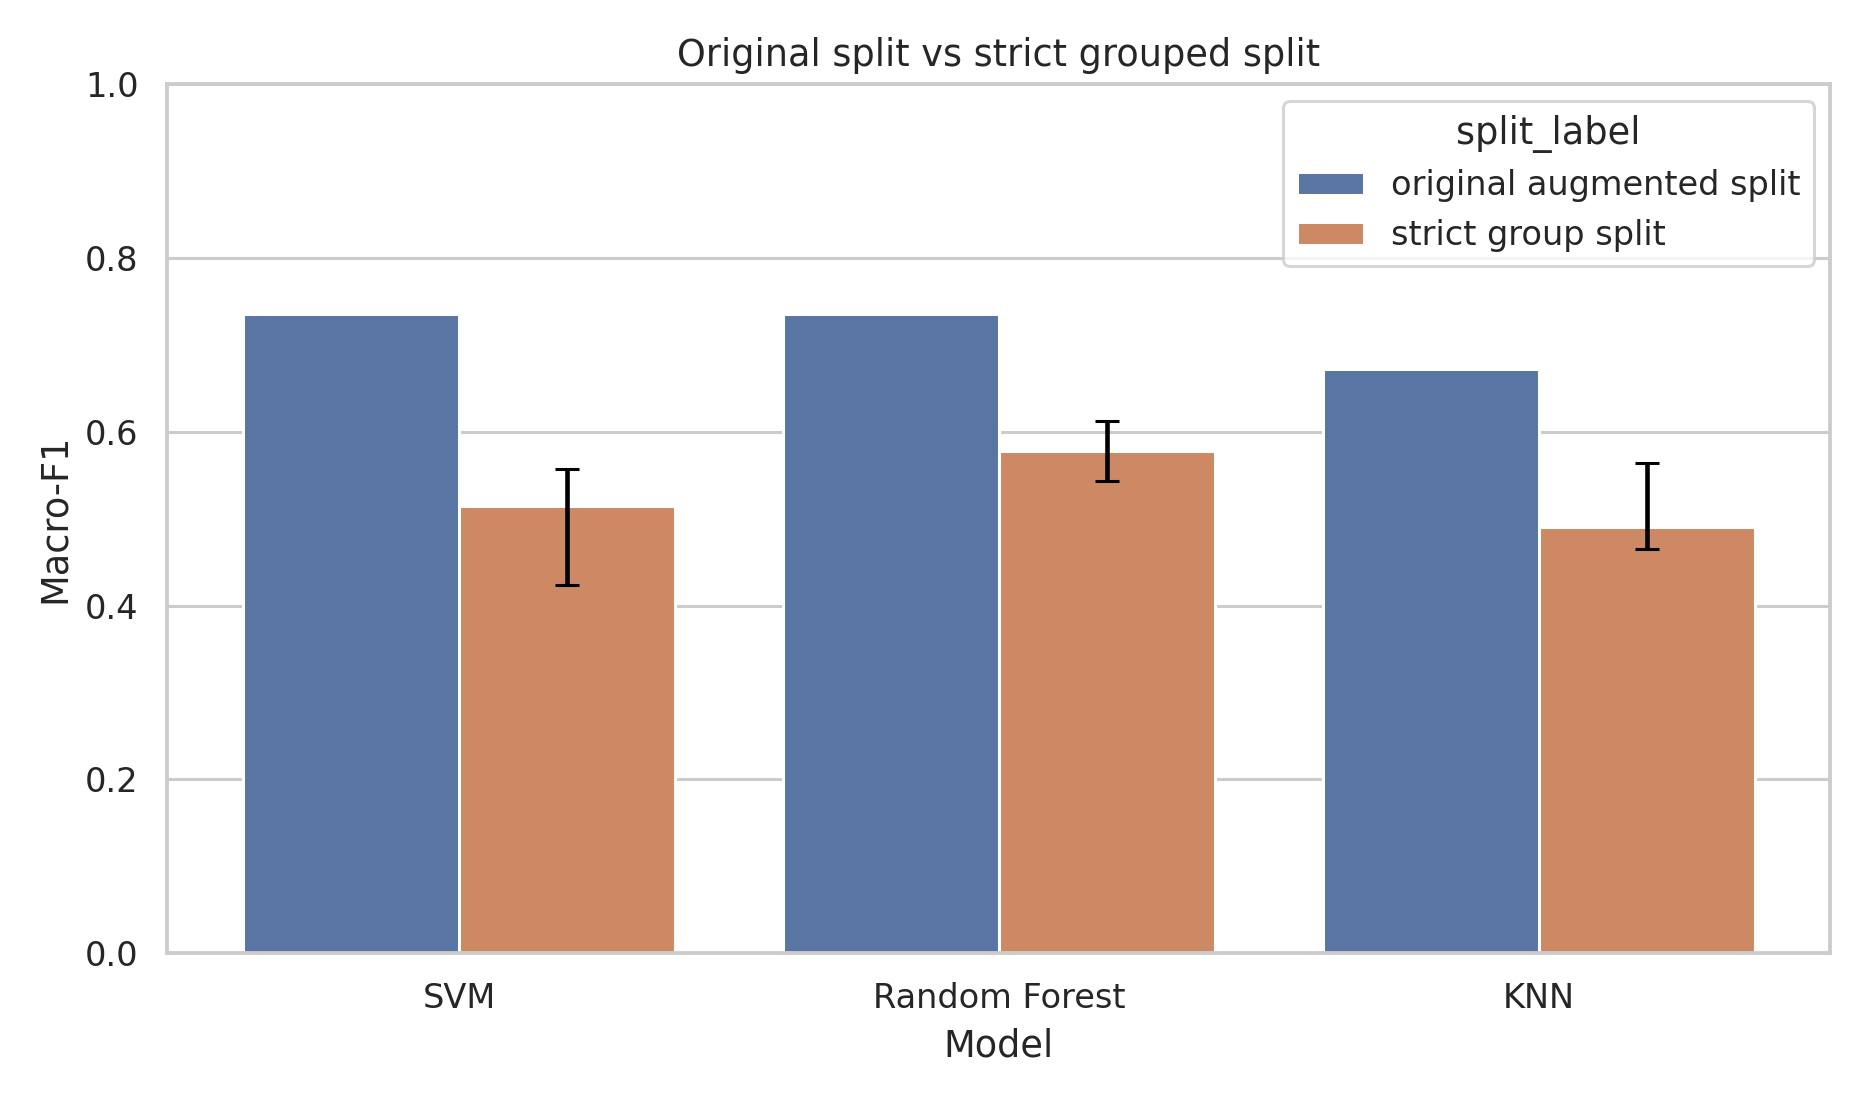
\includegraphics[width=0.82\textwidth]{results_member4/group_split_stability.png}
\caption{原划分与严格分组划分的Macro-F1对比}
\label{fig:group_split_stab}
\end{figure}

\textbf{严格分组划分分析：}
\begin{itemize}
    \item \textbf{性能显著下降}：严格分组划分下，三种模型的Macro-F1均大幅下降。随机森林从0.736降至0.578（$-$0.158），SVM从0.736降至0.515（$-$0.221），KNN从0.672降至0.490（$-$0.182）。这揭示了原增强划分中存在的病灶级信息泄漏使得测试指标偏乐观；
    \item \textbf{随机森林最稳定}：随机森林在严格分组划分下取得最高Macro-F1（0.578）且标准差最小（0.035），再次验证集成方法在数据分布变化下的鲁棒性优势；
    \item \textbf{KNN方差最大}：KNN的标准差最大（0.067），表明其对训练/测试集构成的敏感度最高，这与其基于实例的非参数特性一致；
    \item \textbf{临床意义}：严格分组划分下的性能更能反映算法在真实场景（对全新病灶进行分类）中的预期表现，建议在后续研究中优先采用此划分方式评估模型。
\end{itemize}

\subsection{最差情况分析}

图\ref{fig:worst_cm}展示了所有模型在所有扰动条件下的最差混淆矩阵，即模型表现最脆弱的情境。

\begin{figure}[H]
\centering
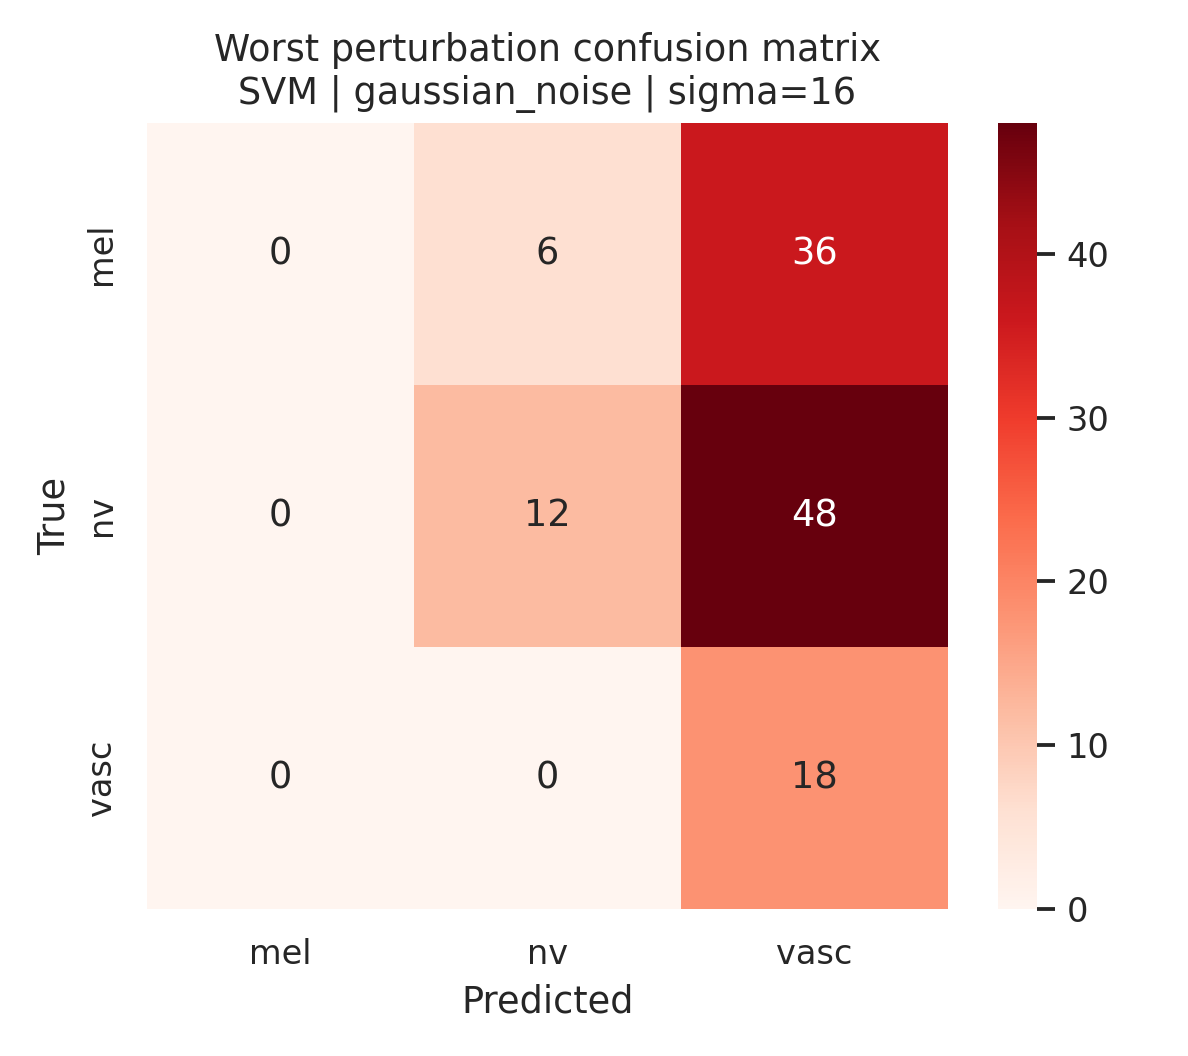
\includegraphics[width=0.55\textwidth]{results_member4/worst_perturbation_confusion_matrix.png}
\caption{最差扰动条件下的混淆矩阵}
\label{fig:worst_cm}
\end{figure}

% ====================== 第8章 讨论 ======================
\section{讨论}\label{sec:discussion}

\subsection{传统方法 vs 深度学习方法}

本项目同时实现了传统手工特征+机器学习方案和深度学习迁移学习方案。两种范式的对比如表\ref{tab:paradigm}所示。

\begin{table}[H]
\centering
\caption{传统方法与深度学习方法范式对比}
\label{tab:paradigm}
\small
\begin{tabular}{lp{4.5cm}p{4.5cm}}
\toprule
\textbf{维度} & \textbf{传统方法} & \textbf{深度学习方法} \\
\midrule
特征来源 & 人工设计（颜色矩、直方图、GLCM、LBP） & 自动学习（CNN层级特征） \\
可解释性 & 高（每维特征有明确物理含义） & 低（黑箱特征） \\
数据需求 & 小样本可用 & 需要较多数据或迁移学习 \\
计算开销 & 极低（CPU分钟级） & 较高（需要GPU） \\
性能上界 & 受限于特征设计 & 通常更高 \\
对扰动的鲁棒性 & 依赖特征选择 & 可学习不变性 \\
临床部署 & 容易（模型小，可解释） & 需额外验证 \\
\bottomrule
\end{tabular}
\end{table}

两种范式并非互斥，而是可以互补：
\begin{enumerate}
    \item \textbf{特征融合}：将手工特征与CNN特征拼接后输入分类器，结合两种特征的互补优势；
    \item \textbf{知识蒸馏}：用深度学习模型指导传统模型训练；
    \item \textbf{分阶段部署}：传统方法做初筛，深度学习方法做精判。
\end{enumerate}

\subsection{临床视角分析}

从临床应用角度看，本项目的分类模型需重点关注以下实际问题：

\subsubsection{假阴性的代价}

对于melanoma（黑色素瘤）的诊断，假阴性（将恶性误判为良性）的代价远高于假阳性。从混淆矩阵来看，随机森林对mel的召回率为69.05\%，即约31\%的mel病例被漏诊——这是不可接受的临床性能。提升mel召回率的方法包括：
\begin{itemize}
    \item 调整决策阈值：降低mel类的分类阈值，以增加假阳性为代价提高真阳性率；
    \item 类别加权：为mel类赋予更高的误分类代价；
    \item 特征增强：引入对mel更具判别力的特征（如蓝白幕、不规则条纹等皮肤镜特有征象的定量描述）。
\end{itemize}

\subsubsection{模型校准与置信度}

在CAD系统中，除分类结果外，模型还应输出预测置信度。SVM的概率输出（Platt scaling）和随机森林的投票比例可作为置信度估计，辅助医生判断模型预测的可靠程度。

\subsection{局限性与改进方向}

尽管本项目取得了可观的分类效果，仍存在以下局限性：

\begin{enumerate}
    \item \textbf{数据规模有限}：200张原始图像对于医学图像分类任务偏小。未来可考虑：(a) 使用公开大型皮肤镜数据集（如ISIC 2018/2019/2020，包含数万张图像）；(b) 使用生成对抗网络（GAN）进行数据增强，生成更多样化的训练样本。

    \item \textbf{特征设计的局限}：当前手工特征（颜色矩、直方图、GLCM、LBP）主要描述全局统计特性，缺乏对医学上重要的局部结构（如色素网络、球状结构、条纹等）的定量描述。未来可引入：(a) SIFT/HOG等局部描述子；(b) 基于病灶分割的形状特征；(c) ABCDE法则（不对称性、边界不规则性、颜色多样性、直径、演化）的定量化特征。

    \item \textbf{未利用病灶分割信息}：病灶区域的分割掩膜可提供重要的形状和边界特征，同时可对病灶区域和正常皮肤区域分别提取特征。

    \item \textbf{类别不平衡处理}：当前使用逆频率类别加权，可进一步尝试SMOTE过采样、ADASYN自适应合成采样等方法。

    \item \textbf{集成学习}：三种基分类器（SVM、RF、KNN）的预测结果可通过Stacking或Voting进行融合，有望进一步提升性能。
\end{enumerate}

% ====================== 第9章 结论 ======================
\section{结论}\label{sec:conclusion}

本项目围绕皮肤镜图像三分类任务，系统性地构建并评估了从数据预处理、特征工程到模型训练和鲁棒性分析的完整方案。主要工作总结如下：

\begin{enumerate}
    \item \textbf{数据预处理}：完成了200张原始皮肤镜图像的去噪、去毛发、尺寸和亮度归一化，并通过旋转和翻转生成了400张增强图像，按80/20比例构建了分层划分的训练集（480张）和测试集（120张）。

    \item \textbf{特征工程}：设计了127维颜色+纹理组合特征（颜色矩9维+颜色直方图96维+GLCM纹理12维+LBP纹理10维），通过StandardScaler标准化和PCA降维进行特征预处理。互信息分析和t-SNE可视化验证了特征的有效性和类别可分性。特征组消融实验确认了颜色直方图的主导贡献和纹理特征的互补作用。

    \item \textbf{模型训练与评估}：对SVM（RBF核）、随机森林和KNN三种分类器进行了系统的网格搜索超参数优化和5折交叉验证。在测试集上，随机森林取得73.33\%的准确率（Macro-F1=0.7360），SVM取得72.50\%的准确率（Macro-F1=0.7360），KNN取得66.67\%的准确率（Macro-F1=0.6721）。同时构建了ResNet-18和MobileNetV2深度学习迁移学习方案作为性能上界参考。

    \item \textbf{鲁棒性分析}：从增强图像预测一致性、10种图像扰动下的性能保持、以及严格分组划分的泛化稳定性三个层面，全面评估了各模型的鲁棒性。随机森林在多数扰动和划分变化下表现出最高的稳定性。

    \item \textbf{临床视角分析}：从假阴性代价、模型校准和实际部署等角度探讨了模型向临床应用过渡时需要考虑的关键问题，并提出了包括引入局部结构特征、病灶分割信息、改进类别不平衡处理等改进方向。
\end{enumerate}

实验结果表明，基于手工颜色和纹理特征的传统机器学习方法在皮肤镜图像分类中能够取得有意义的分类精度（约73\%），其中颜色分布信息是最具判别力的特征类型。然而，mel与nv之间的高混淆率（mel召回率仅约69\%）提示了手工特征在捕捉细微视觉差异方面的局限性。深度学习方法有望通过自动学习更具判别力的特征表示来突破这一瓶颈。通过鲁棒性分析验证，本项目的方法对常见的图像质量变化具有一定容忍度，但在强噪声和大角度旋转下性能存在明显衰减，这也是未来工作需要重点解决的问题。

% ====================== 参考文献 ======================
\begin{thebibliography}{99}

\bibitem{isic}
Tschandl, P., Rosendahl, C., \& Kittler, H. (2018).
The HAM10000 dataset, a large collection of multi-source dermatoscopic images of common pigmented skin lesions.
\textit{Scientific Data}, 5, 180161.

\bibitem{esteva}
Esteva, A., Kuprel, B., Novoa, R. A., et al. (2017).
Dermatologist-level classification of skin cancer with deep neural networks.
\textit{Nature}, 542(7639), 115–118.

\bibitem{haralick}
Haralick, R. M., Shanmugam, K., \& Dinstein, I. (1973).
Textural features for image classification.
\textit{IEEE Transactions on Systems, Man, and Cybernetics}, SMC-3(6), 610–621.

\bibitem{ojala}
Ojala, T., Pietikäinen, M., \& Mäenpää, T. (2002).
Multiresolution gray-scale and rotation invariant texture classification with local binary patterns.
\textit{IEEE Transactions on Pattern Analysis and Machine Intelligence}, 24(7), 971–987.

\bibitem{he2016}
He, K., Zhang, X., Ren, S., \& Sun, J. (2016).
Deep residual learning for image recognition.
\textit{Proceedings of the IEEE Conference on Computer Vision and Pattern Recognition (CVPR)}, 770–778.

\bibitem{sandler}
Sandler, M., Howard, A., Zhu, M., Zhmoginov, A., \& Chen, L. C. (2018).
MobileNetV2: Inverted residuals and linear bottlenecks.
\textit{Proceedings of the IEEE Conference on Computer Vision and Pattern Recognition (CVPR)}, 4510–4520.

\bibitem{strickland}
Strickland, R. N., \& Hahn, H. (1994).
Wavelet transform matched filters for the detection of stellate lesions in mammograms.
\textit{Proceedings of the IEEE International Conference on Image Processing (ICIP)}.

\bibitem{lecun}
LeCun, Y., Bengio, Y., \& Hinton, G. (2015).
Deep learning.
\textit{Nature}, 521(7553), 436–444.

\bibitem{breiman}
Breiman, L. (2001).
Random forests.
\textit{Machine Learning}, 45(1), 5–32.

\bibitem{cortes}
Cortes, C., \& Vapnik, V. (1995).
Support-vector networks.
\textit{Machine Learning}, 20(3), 273–297.

\bibitem{pca}
Jolliffe, I. T. (2002).
\textit{Principal Component Analysis} (2nd ed.).
Springer.

\bibitem{maaten}
van der Maaten, L., \& Hinton, G. (2008).
Visualizing data using t-SNE.
\textit{Journal of Machine Learning Research}, 9, 2579–2605.

\bibitem{isic_challenge}
Codella, N. C. F., Gutman, D., Celebi, M. E., et al. (2018).
Skin lesion analysis toward melanoma detection: A challenge at the 2017 International Symposium on Biomedical Imaging (ISBI).
\textit{arXiv preprint arXiv:1710.05006}.

\end{thebibliography}

% ====================== 团队分工 ======================
\section*{团队分工说明}
\addcontentsline{toc}{section}{团队分工说明}

本项目由五名成员协作完成，各成员具体贡献如下：

\begin{table}[H]
\centering
\caption{小组成员分工明细}
\begin{tabular}{llp{8cm}}
\toprule
\textbf{成员} & \textbf{模块} & \textbf{具体工作内容} \\
\midrule
成员1 & 数据与预处理 &
\tabincell{l}{数据集整理、格式统一、路径管理；\\ 图像尺寸归一化；去噪、去毛发、亮度归一化；\\ 训练集/测试集划分；输出可训练的标准数据集} \\
\midrule
成员2 & 颜色特征+纹理特征工程 &
\tabincell{l}{提取颜色特征（颜色矩、颜色直方图）；\\ 提取纹理特征（GLCM、LBP）；\\ 特征拼接、归一化、PCA降维；\\ 特征有效性分析（互信息、t-SNE、消融实验）} \\
\midrule
成员3 & 传统机器学习模型训练与评估 &
\tabincell{l}{SVM / 随机森林 / KNN 模型搭建；\\ 交叉验证、网格搜索参数调优；\\ 在原始图像上测试并计算指标；\\ 输出准确率、精确率、召回率、F1、混淆矩阵} \\
\midrule
成员4 & 增强数据鲁棒性测试 &
\tabincell{l}{在400张增强图像上测试传统模型；\\ 对比原图与增强图的性能差异；\\ 分析算法稳定性与抗干扰能力（10种扰动）；\\ 完成严格分组划分稳定性分析} \\
\midrule
成员5 & 深度学习对比实验 &
\tabincell{l}{使用ResNet18/MobileNetV2迁移学习分类；\\ 训练、验证、测试全流程；\\ 深度模型在原图与增强图上的表现分析；\\ 传统方法 vs 深度学习对比分析} \\
\bottomrule
\end{tabular}
\end{table}

\textit{说明：每位成员均实质性参与了代码编写、实验执行与结果分析工作，符合课程对每位成员必须从事实质性工作的要求。}

% ====================== 附录 ======================
\appendix
\section{项目代码结构}

完整的项目代码目录结构如下：

{\small\begin{verbatim}
project/
├── deep_learning/              # 深度学习模块
│   ├── main.py                 # 深度学习实验入口
│   ├── config.py               # 配置（路径、超参数）
│   ├── dataset.py              # 数据加载与预处理
│   ├── models.py               # ResNet-18 / MobileNetV2 构建
│   ├── train.py                # 训练与验证循环
│   ├── evaluate.py             # 测试集评估
│   ├── visualize.py            # 训练曲线与错例可视化
│   ├── predict.py              # 推理与输出生成
│   └── utils.py                # 工具函数
│
└── final_project/              # 传统方法模块
    ├── train/                  # 训练集图像 (480张)
    ├── test/                   # 测试集图像 (120张)
    ├── features/               # 特征文件
    │   ├── X_train_norm.npy    # 训练集归一化特征
    │   ├── X_test_norm.npy     # 测试集归一化特征
    │   ├── X_train_pca.npy     # PCA降维后特征
    │   ├── X_test_pca.npy      # PCA降维后特征
    │   ├── scaler.pkl          # StandardScaler
    │   ├── pca.pkl             # PCA模型
    │   └── feature_names.npy   # 特征名称
    ├── results/                # 模型评估结果
    │   ├── best_model_SVM.pkl  # 最优SVM模型
    │   ├── model_comparison.csv # 模型对比表
    │   └── *.png               # 可视化图表
    ├── results_member4/        # 鲁棒性分析结果
    ├── feature_extraction.py   # 特征提取脚本
    ├── feature_analysis.py     # 特征分析脚本
    ├── model_training.py       # 模型训练脚本
    └── robustness_analysis.py  # 鲁棒性分析脚本
\end{verbatim}}

\section{实验环境}

\begin{table}[H]
\centering
\caption{实验软件环境}
\small
\begin{tabular}{lp{7cm}}
\toprule
\textbf{组件} & \textbf{版本/说明} \\
\midrule
操作系统 & Windows 11 \\
Python & 3.12 \\
NumPy & 数值计算与特征矩阵存储 \\
Pandas & 标签读取与结果汇总 \\
scikit-learn & ML算法实现（SVM, RF, KNN, PCA, GridSearchCV等） \\
scikit-image & 图像特征提取（GLCM, LBP） \\
OpenCV & 图像读取与颜色空间转换 \\
Matplotlib \& Seaborn & 数据可视化 \\
PyTorch & 深度学习框架（ResNet-18, MobileNetV2） \\
Pillow & 图像扰动处理 \\
\bottomrule
\end{tabular}
\end{table}

\section{LaTeX 编译说明}

本报告使用 \texttt{pdflatex} 编译（需安装完整 TeX Live 或 MiKTeX 发行版）：

\begin{verbatim}
pdflatex experiment_report.tex
pdflatex experiment_report.tex   # 第二次编译生成目录和交叉引用
\end{verbatim}

\end{document}
